\documentclass{article}

\usepackage[utf8]{inputenc}

\usepackage{amsmath, bm}
\usepackage{graphicx}
\usepackage{amssymb}
\usepackage{float}
\usepackage{caption}
\usepackage{subcaption}
\usepackage{hyperref}
\usepackage{tikz}
\usepackage{layout}
\usepackage{booktabs}

\usepackage[margin=1in]{geometry}
\usepackage{listings}
\usepackage{xcolor}
\usepackage{color, colortbl}
\usepackage{textgreek}
\usepackage{mathrsfs}
\usepackage{savetrees}

\usetikzlibrary{calc}
\usetikzlibrary{angles,quotes} % for pic
\usetikzlibrary{patterns,snakes}
\usetikzlibrary{arrows}
\tikzset{>=latex} % for LaTeX arrow head

\setlength{\parskip}{\baselineskip}%
\setlength{\parindent}{0pt}%
\linespread{0.9}


\definecolor{codegreen}{rgb}{0,0.6,0}
\definecolor{codegray}{rgb}{0.5,0.5,0.5}
\definecolor{codepurple}{rgb}{0.58,0,0.82}
\definecolor{backcolour}{rgb}{0.95,0.95,0.92}

\lstdefinestyle{mystyle}{
    backgroundcolor=\color{backcolour},   
    commentstyle=\color{codegreen},
    keywordstyle=\color{magenta},
    numberstyle=\tiny\color{codegray},
    stringstyle=\color{codepurple},
    basicstyle=\ttfamily\footnotesize,
    breakatwhitespace=false,         
    breaklines=true,                 
    captionpos=b,                    
    keepspaces=true,                 
    numbers=left,                    
    numbersep=5pt,                  
    showspaces=false,                
    showstringspaces=false,
    showtabs=false,                  
    tabsize=2
}

\lstset{style=mystyle}



\begin{document}

\title{Computational Fluid Dynamics \\
    \large Interim Report}
\author{lwp26}
\date{October 2024}
\maketitle 

\iffalse
\begin{abstract}
    \centering

\end{abstract}
\fi

%-----------------------------------------------------------------------------------------
\section{Introduction}
%-----------------------------------------------------------------------------------------

\section{Software}

The software is a Qt application that calls fortran subroutines to solve the Euler equations for a 2D inviscid flow. The user interface is shown in Figure \ref{fig:ui}.


\section{Discussion}

% Comment on the results from the above two test cases. Pay special attention to ways of
% assessing the accuracy of the solutions and further figures that you can create to analyse this

% Discuss the effects of varying CFL number, smoothing factor and mesh size. Examine how
% these choices affect accuracy, stability and runtime of the solver.

Higher values of ni tested caused a fatal exception in chkstk.asm which indicated that the program ran out of stack space when allocating the grid arrays.
This was resolved by increasing the stack size in the compiler options.

% for each figure
% explain trend
% explain magnitude
\subsection{Bump case}

Figure \ref{fig:bump_mach} shows the Mach number distribution over the bump domain.

Figure \ref{fig:bump_cp}

Figure \ref{fig:bump_conv}

Figure \ref{fig:bump_d_avg_cfl}

Figure \ref{fig:bump_time_cfl}

Figure \ref{fig:bump_d_avg_ni}

Figure \ref{fig:bump_time_ni}

Figure \ref{fig:bump_cfl_sfac_residual}

Figure \ref{fig:bump_cfl_sfac_time}

\subsection{Bend case}

Figure \ref{fig:bend_mach}

Figure \ref{fig:bend_cp}

Figure \ref{fig:bend_conv}

Figure \ref{fig:bend_cfl_sfac_residual}

Figure \ref{fig:bend_cfl_sfac_time}



\section{Appendix}

\begin{figure}[H]
    \centering
    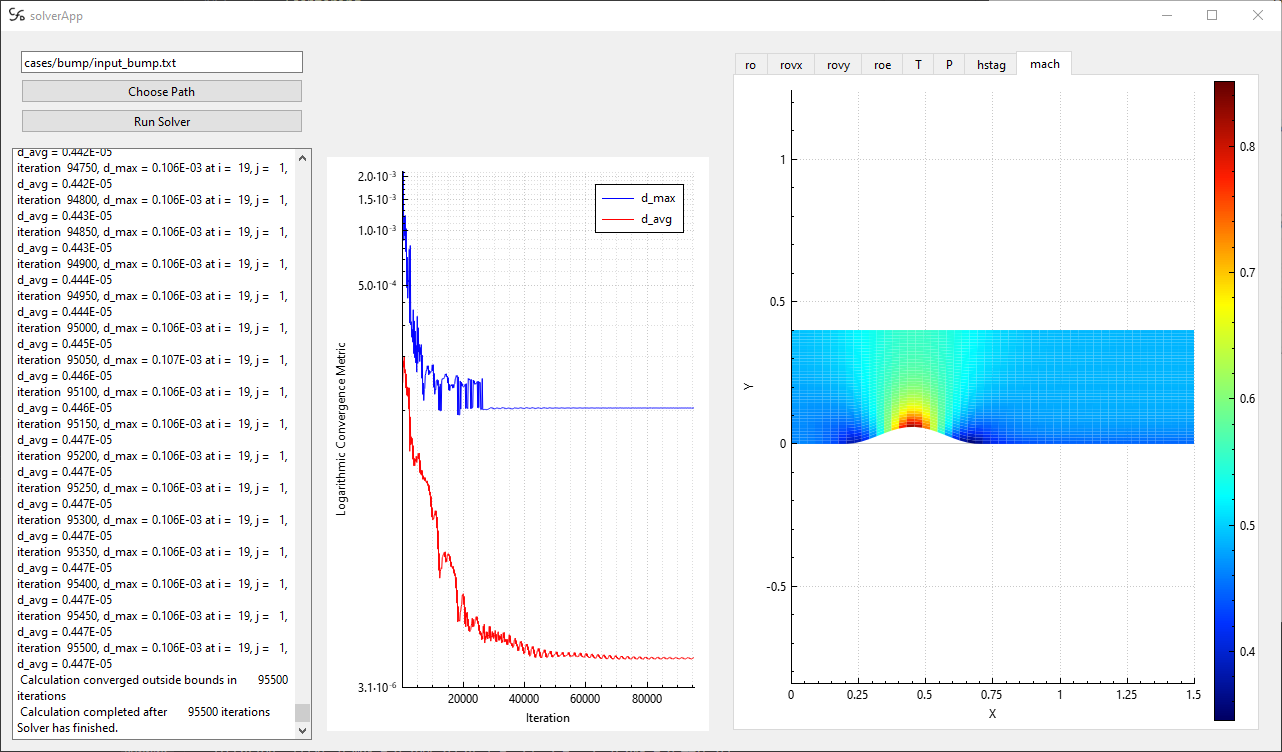
\includegraphics[width=0.8\textwidth]{figures/software.png}
    \caption{The user interface of the software.}
    \label{fig:ui}
\end{figure}

\subsection{Bump test case}

\begin{figure}[H]
    \centering
    \begin{subfigure}{0.99\textwidth}
        \centering
        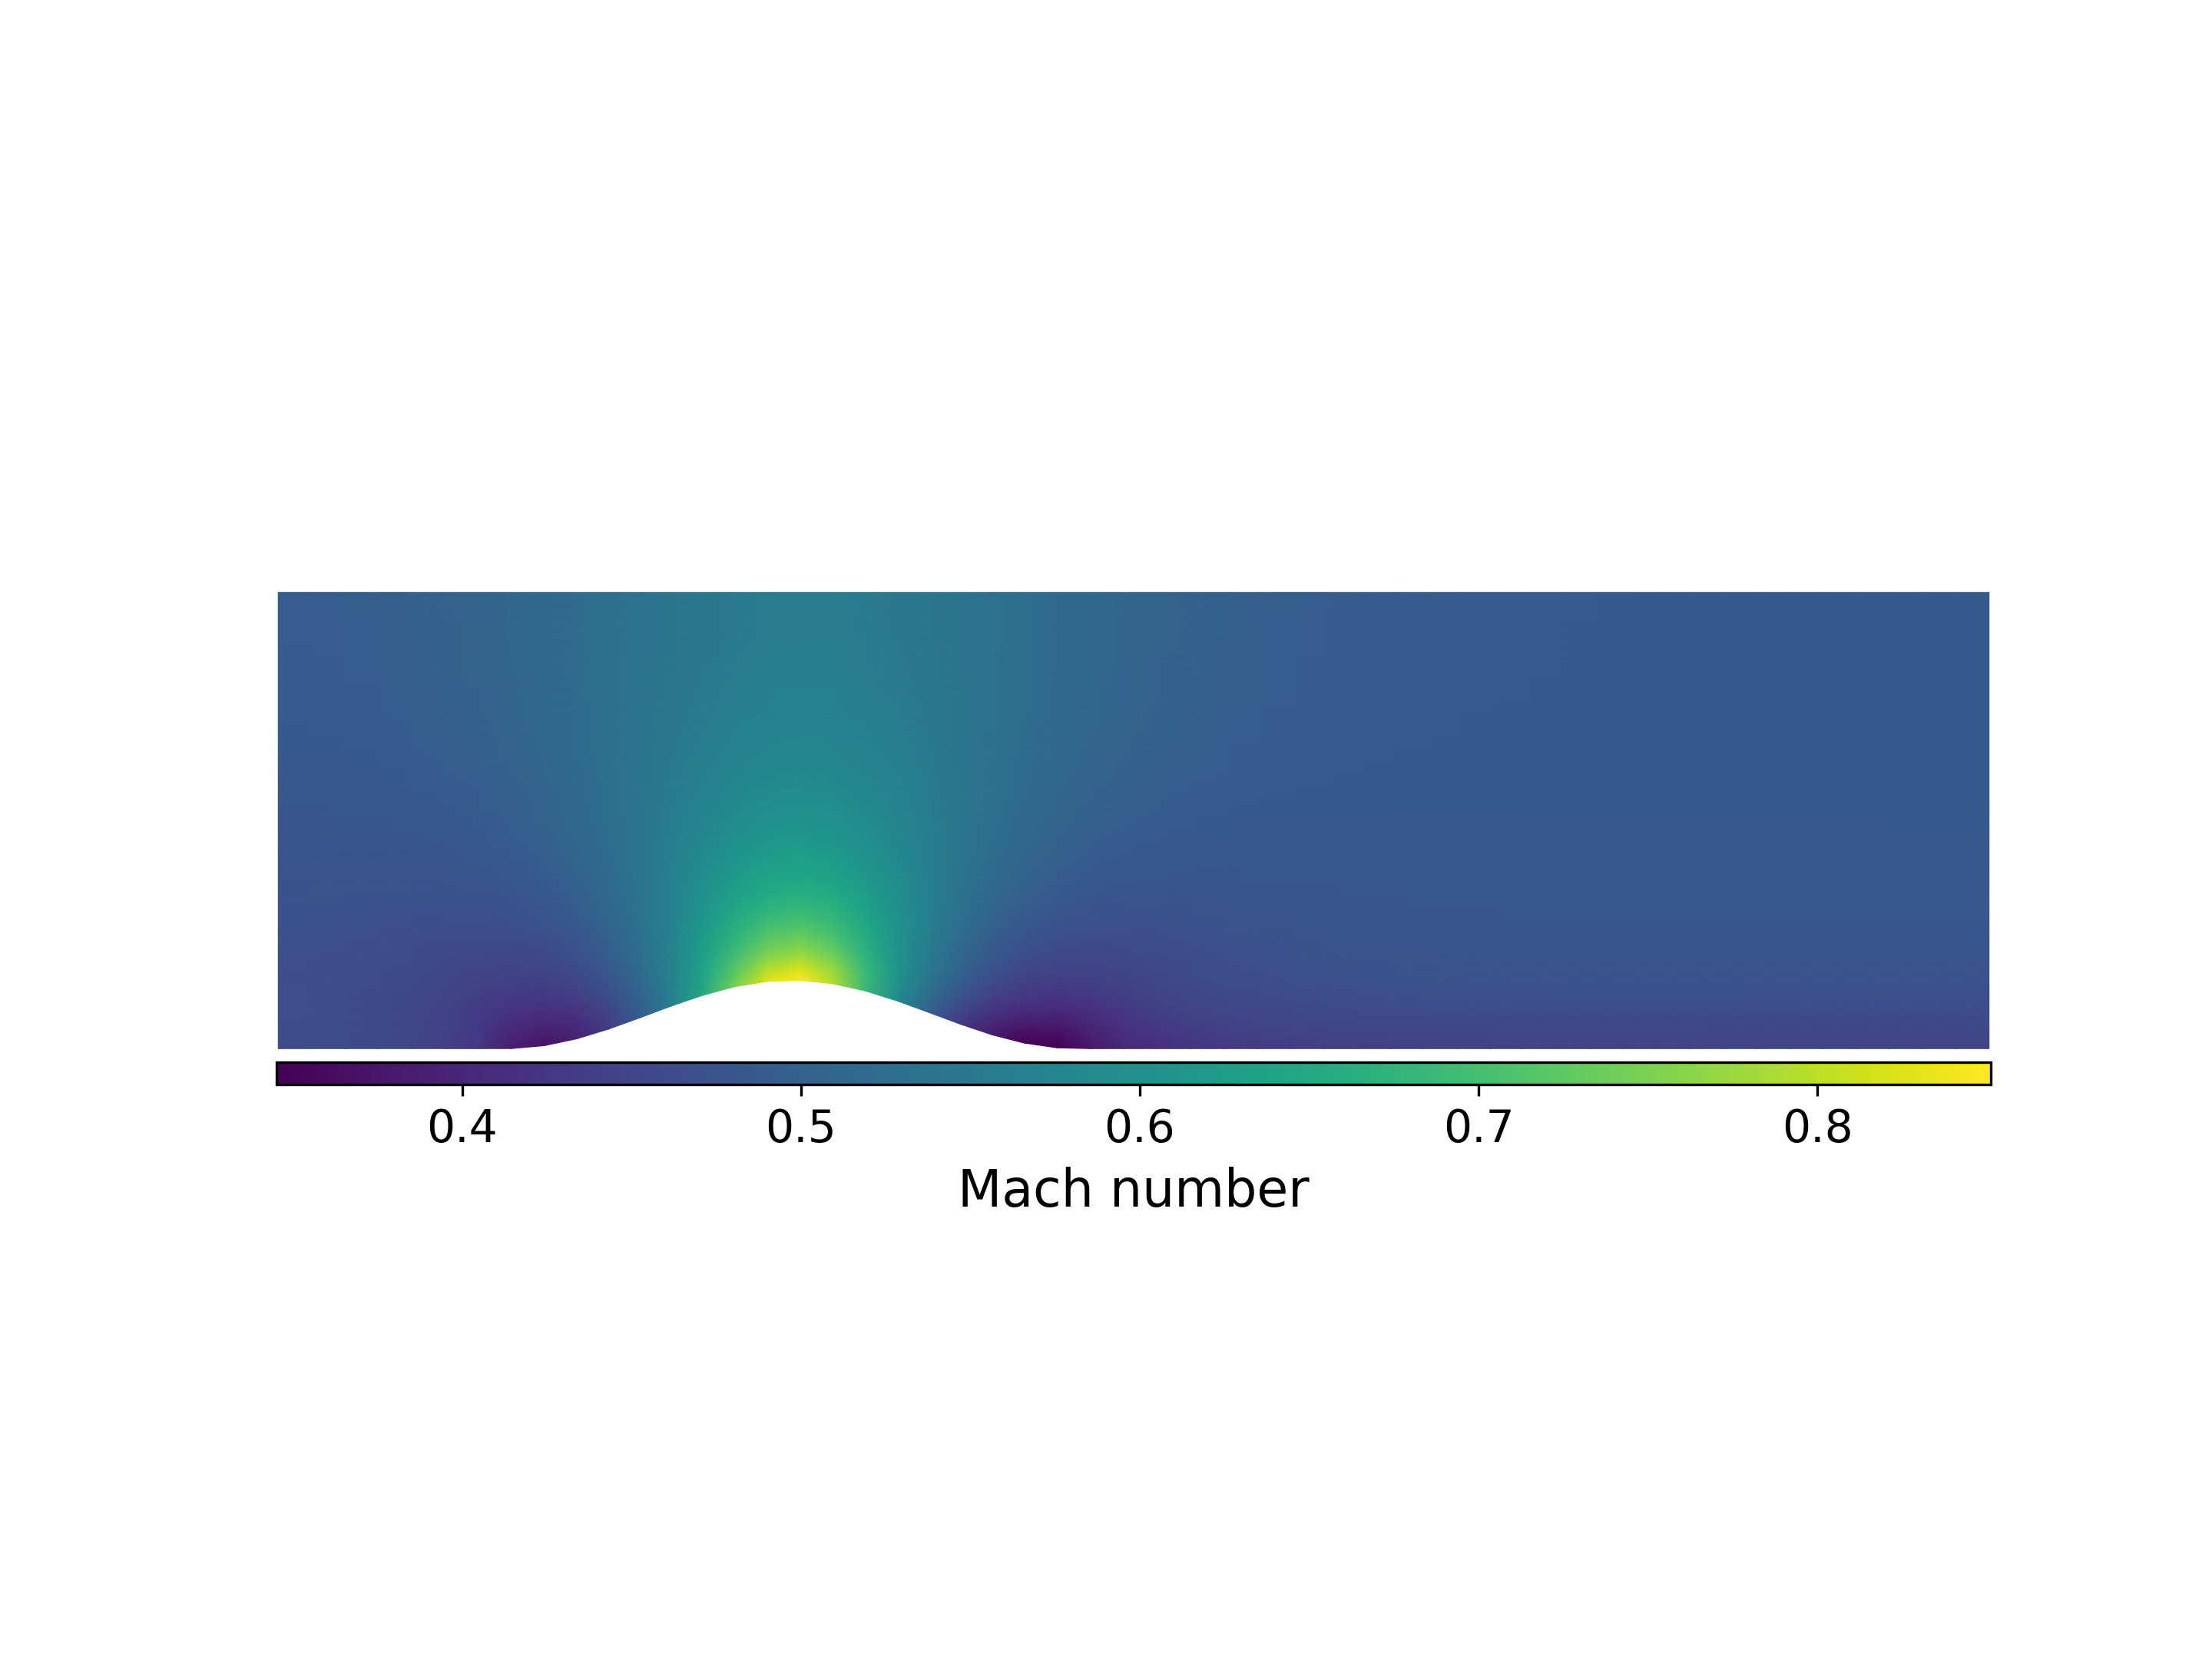
\includegraphics[width=0.7\textwidth]{figures/bump_mach.png}
        \caption{}
        \label{fig:bump_mach}
    \end{subfigure}
    \begin{subfigure}{0.99\textwidth}
        \centering
        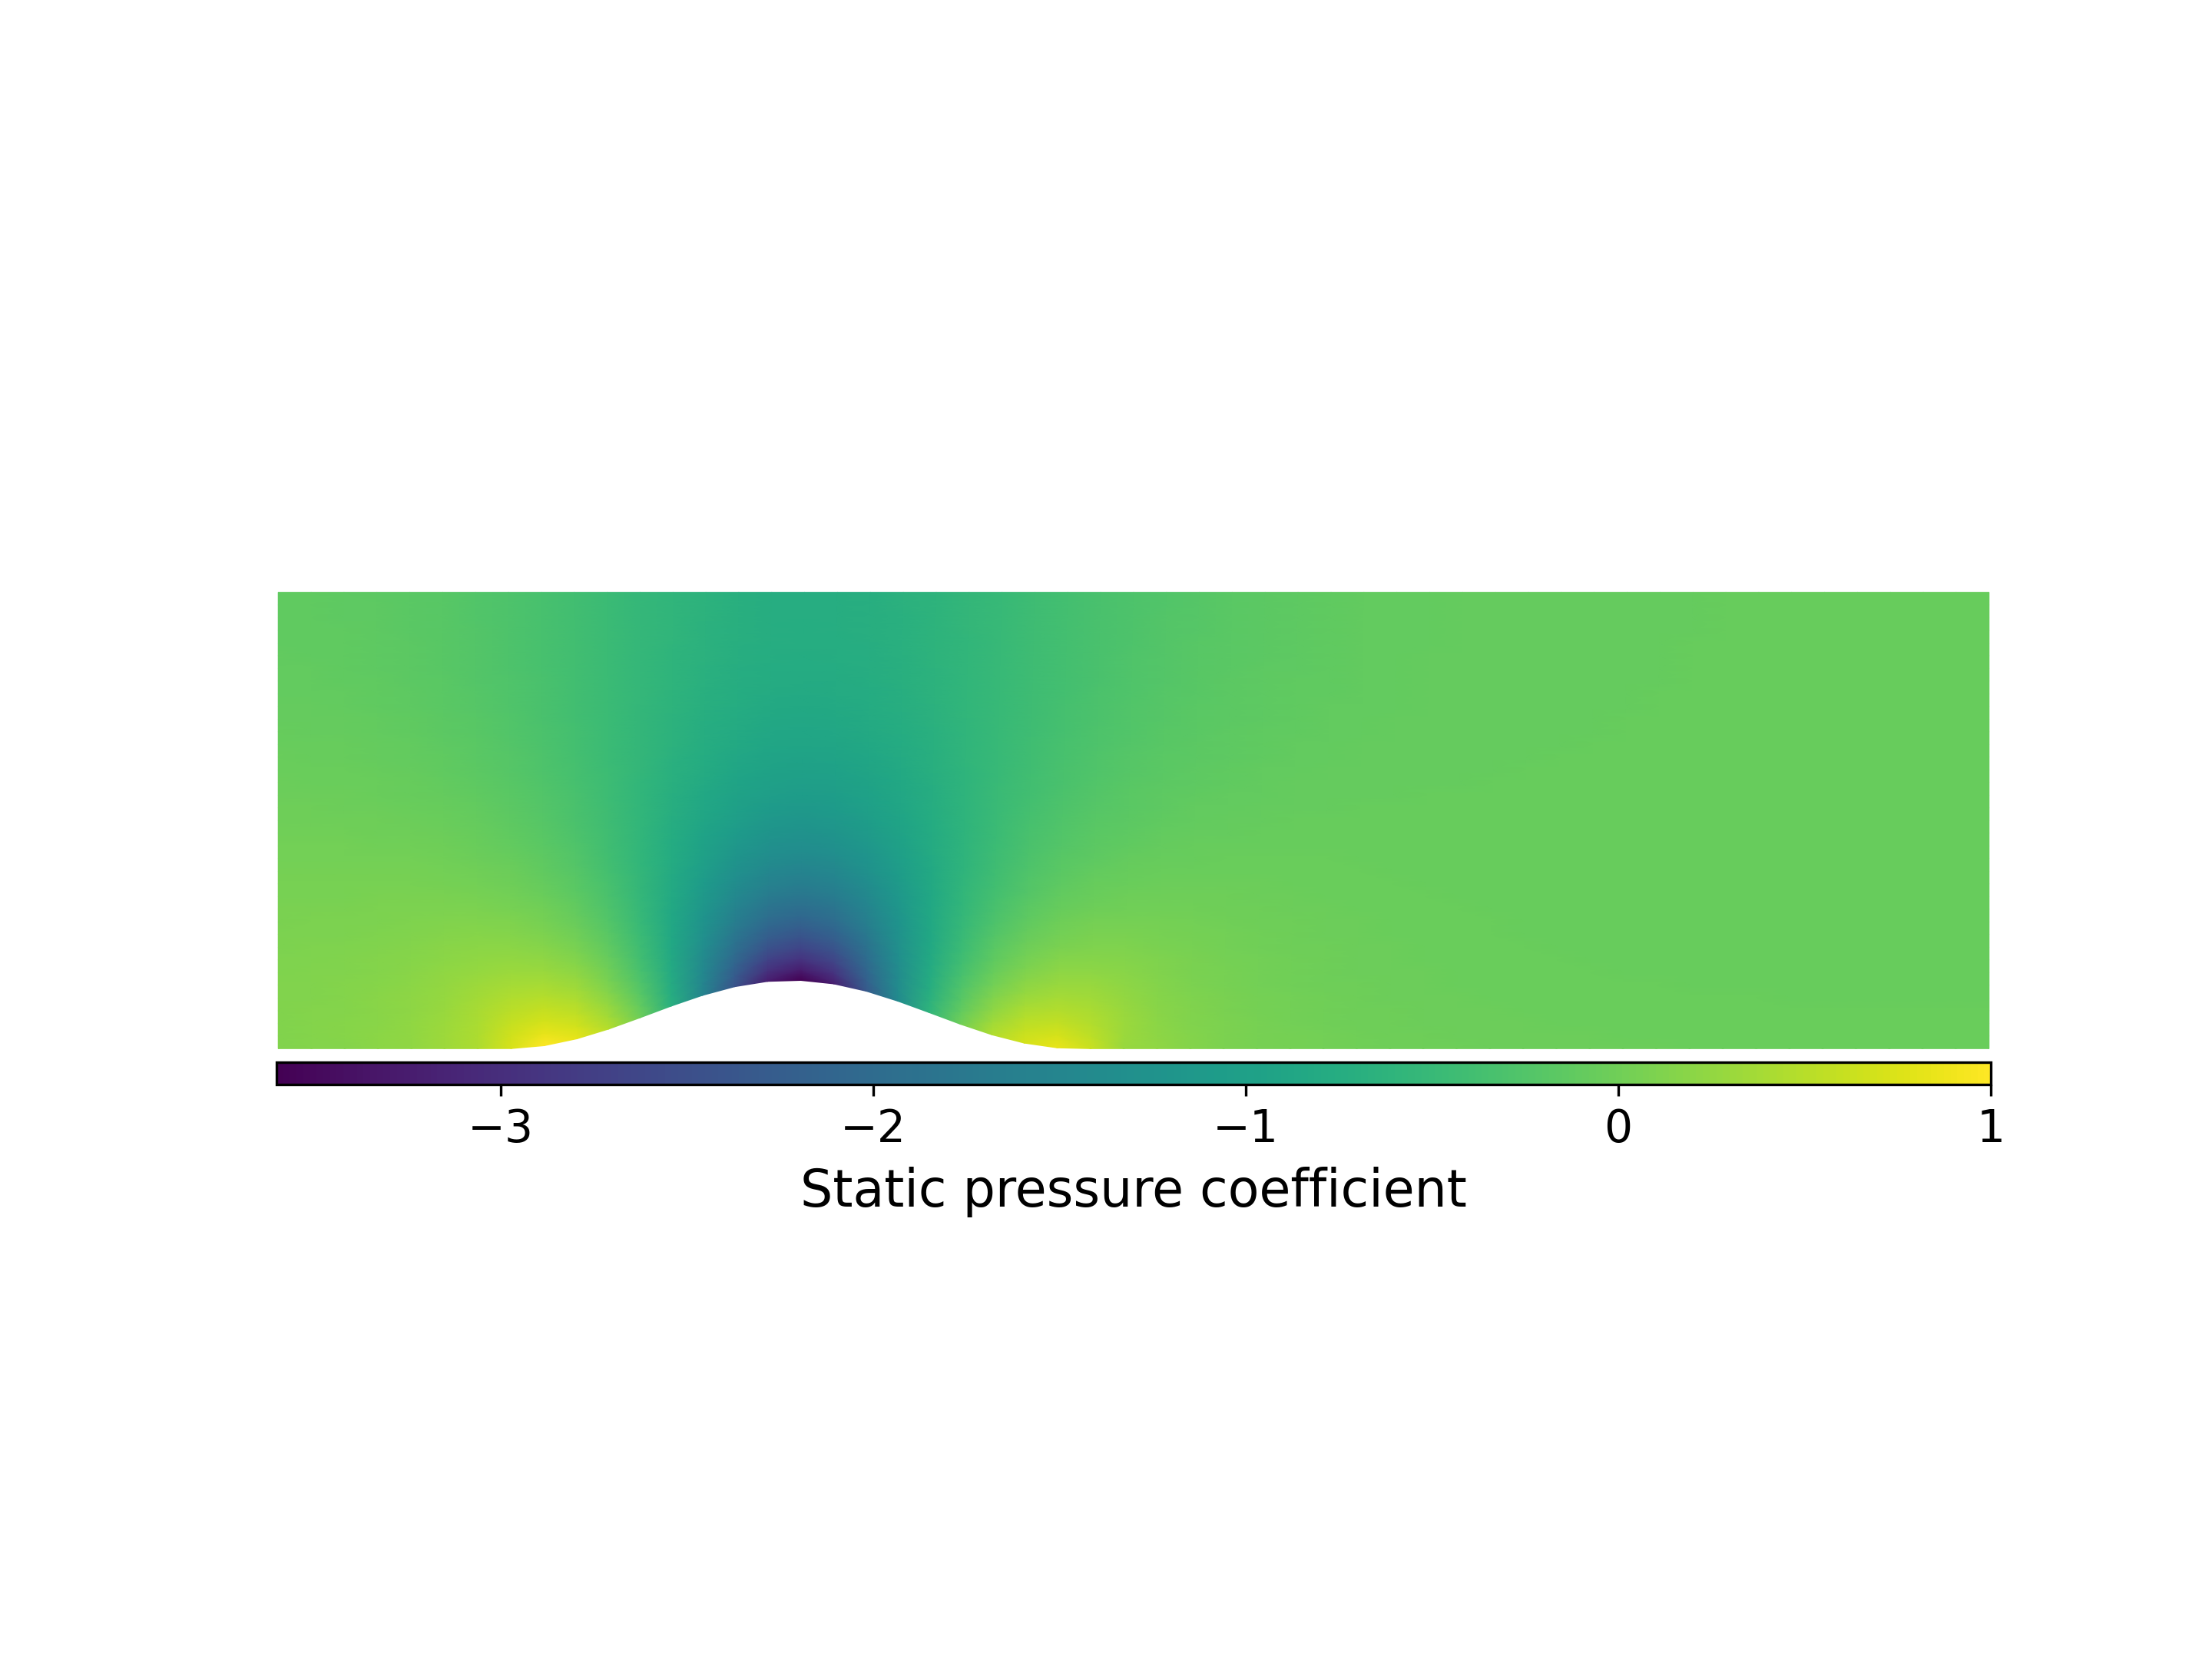
\includegraphics[width=0.7\textwidth]{figures/bump_cp.png}
        \caption{}
        \label{fig:bump_cp}
    \end{subfigure}
    \caption{Bump test case results $CFL = 0.05$, $sfac = 0.1$, $n_i = 53$, $n_j = 37$. Converged in 95500 iterations.}
\end{figure}

\begin{figure}[H]
    \centering
    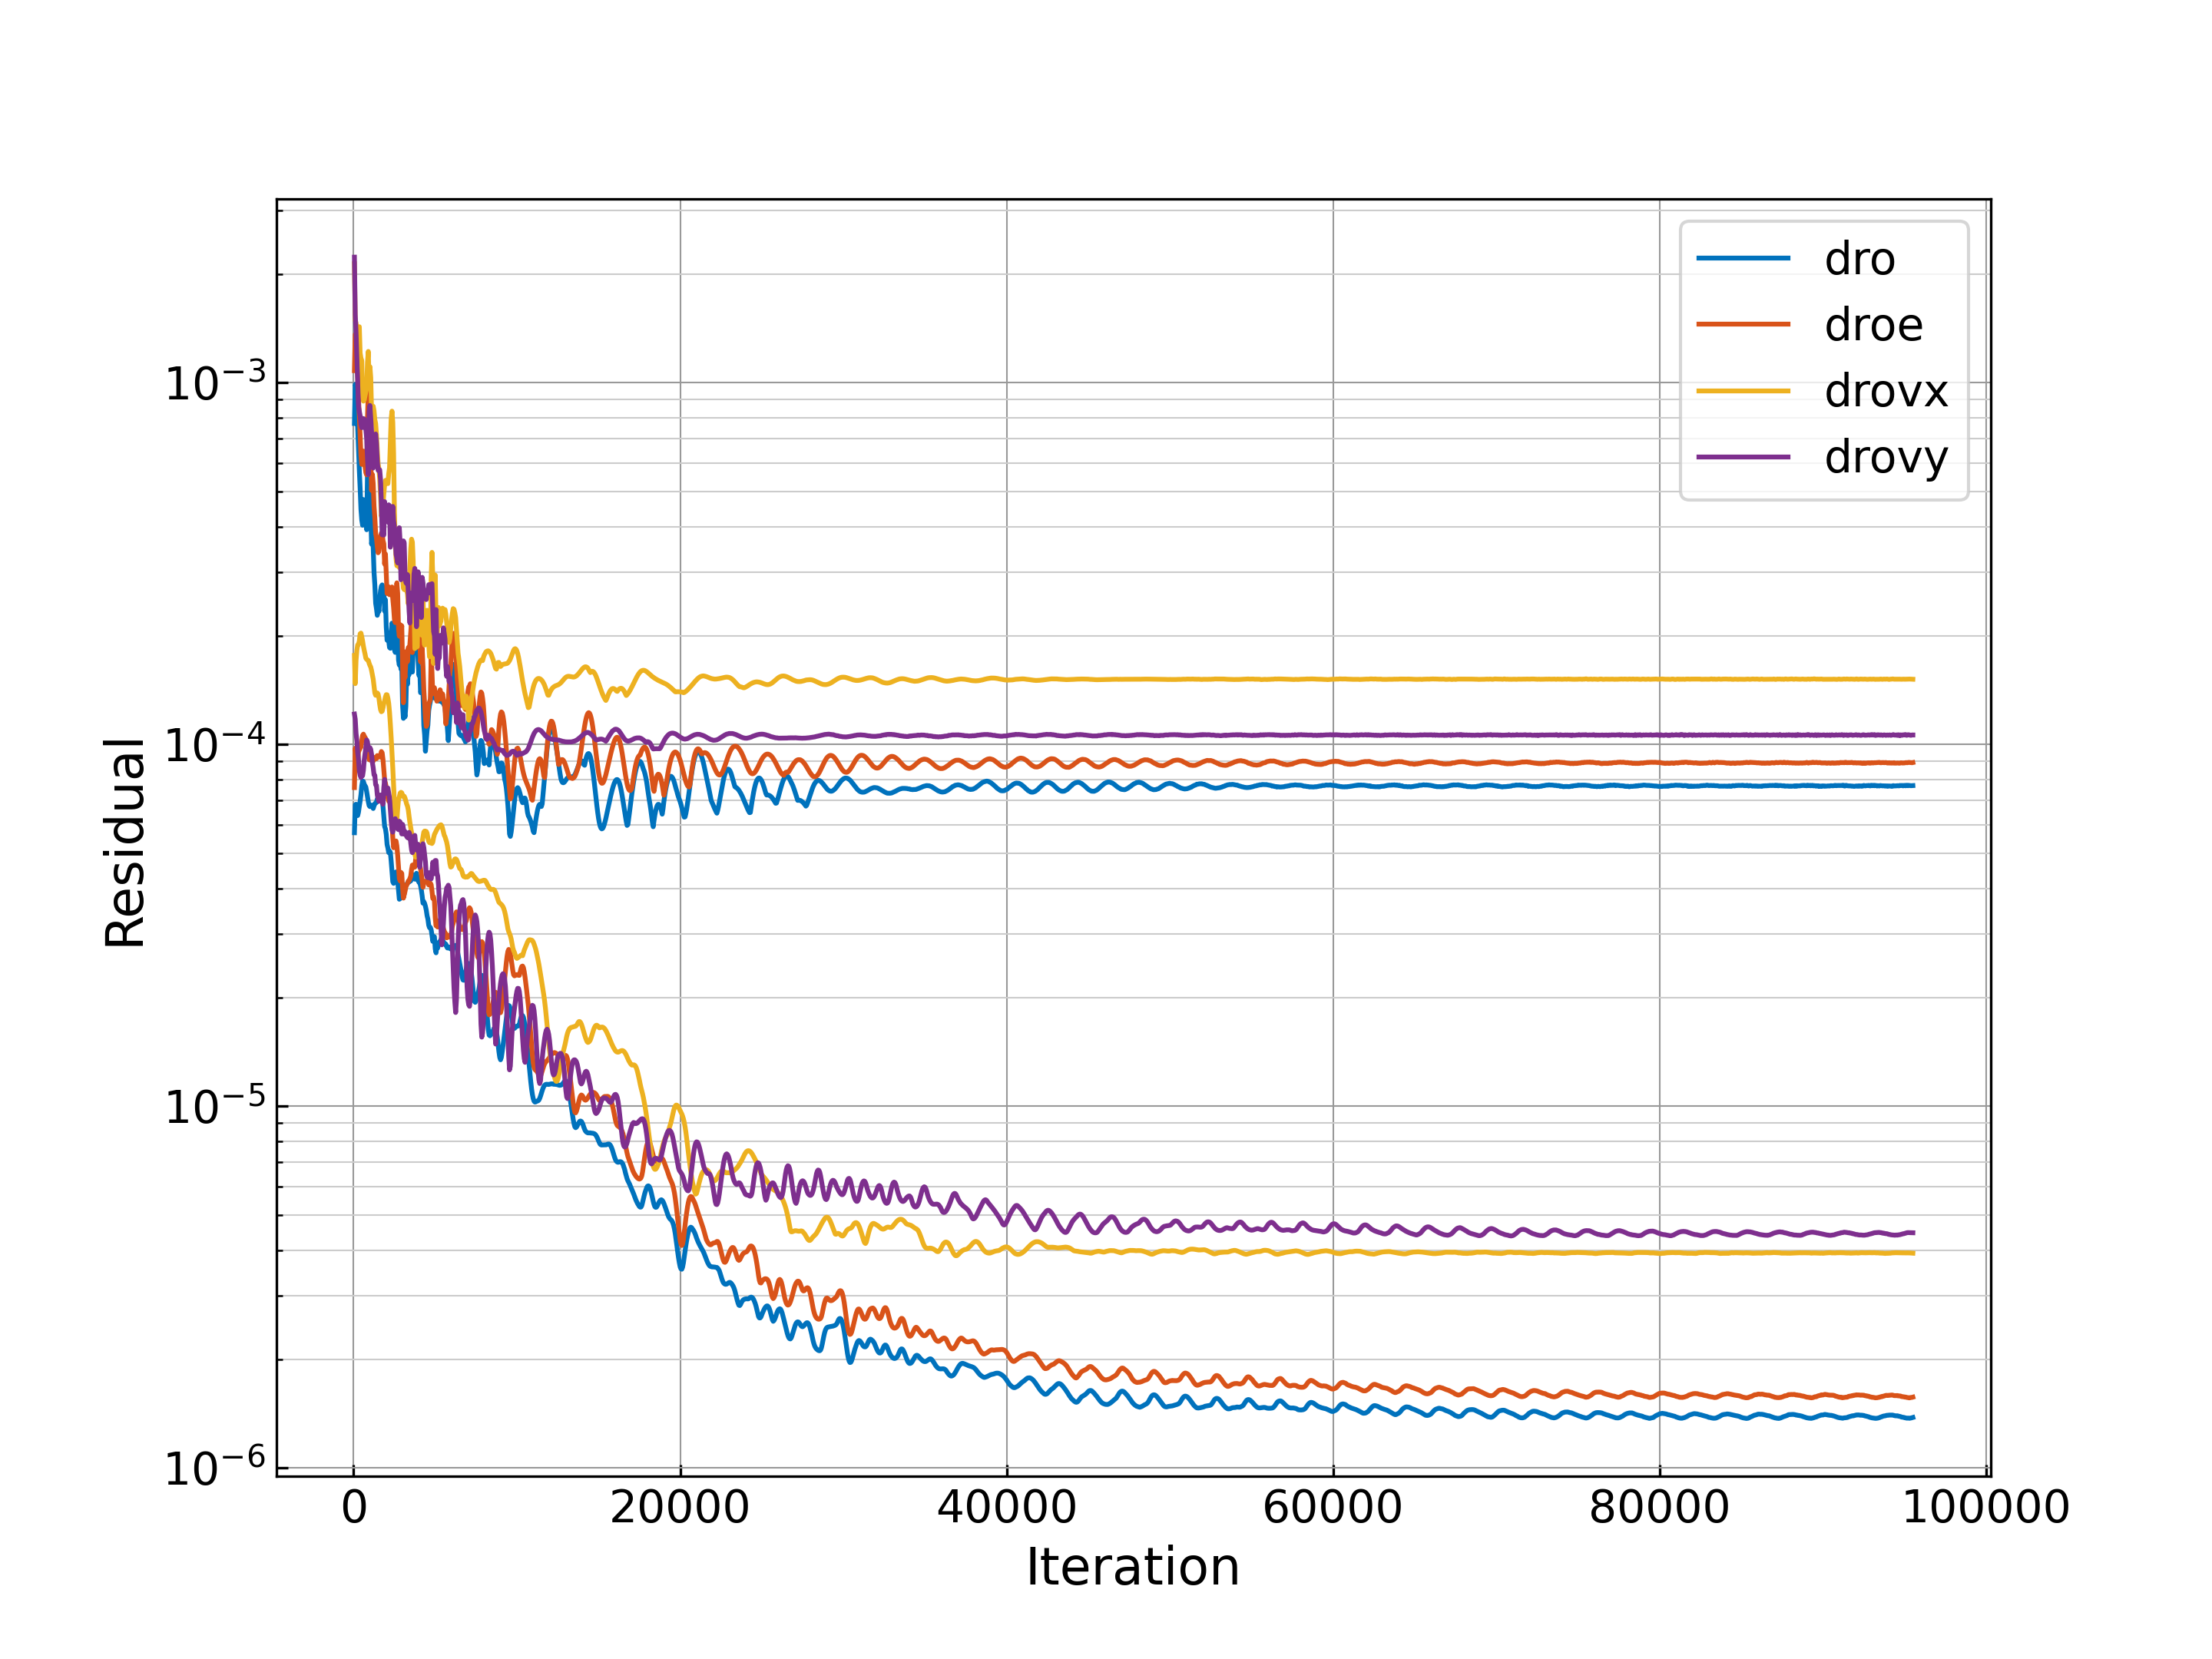
\includegraphics[width=0.8\textwidth]{figures/bump_conv.png}
    \caption{Convergence history of primary flow variables for the bump case}
    \label{fig:bump_conv}
\end{figure}

\begin{figure}[H]
    \centering
    \begin{subfigure}{0.49\textwidth}
        \centering
        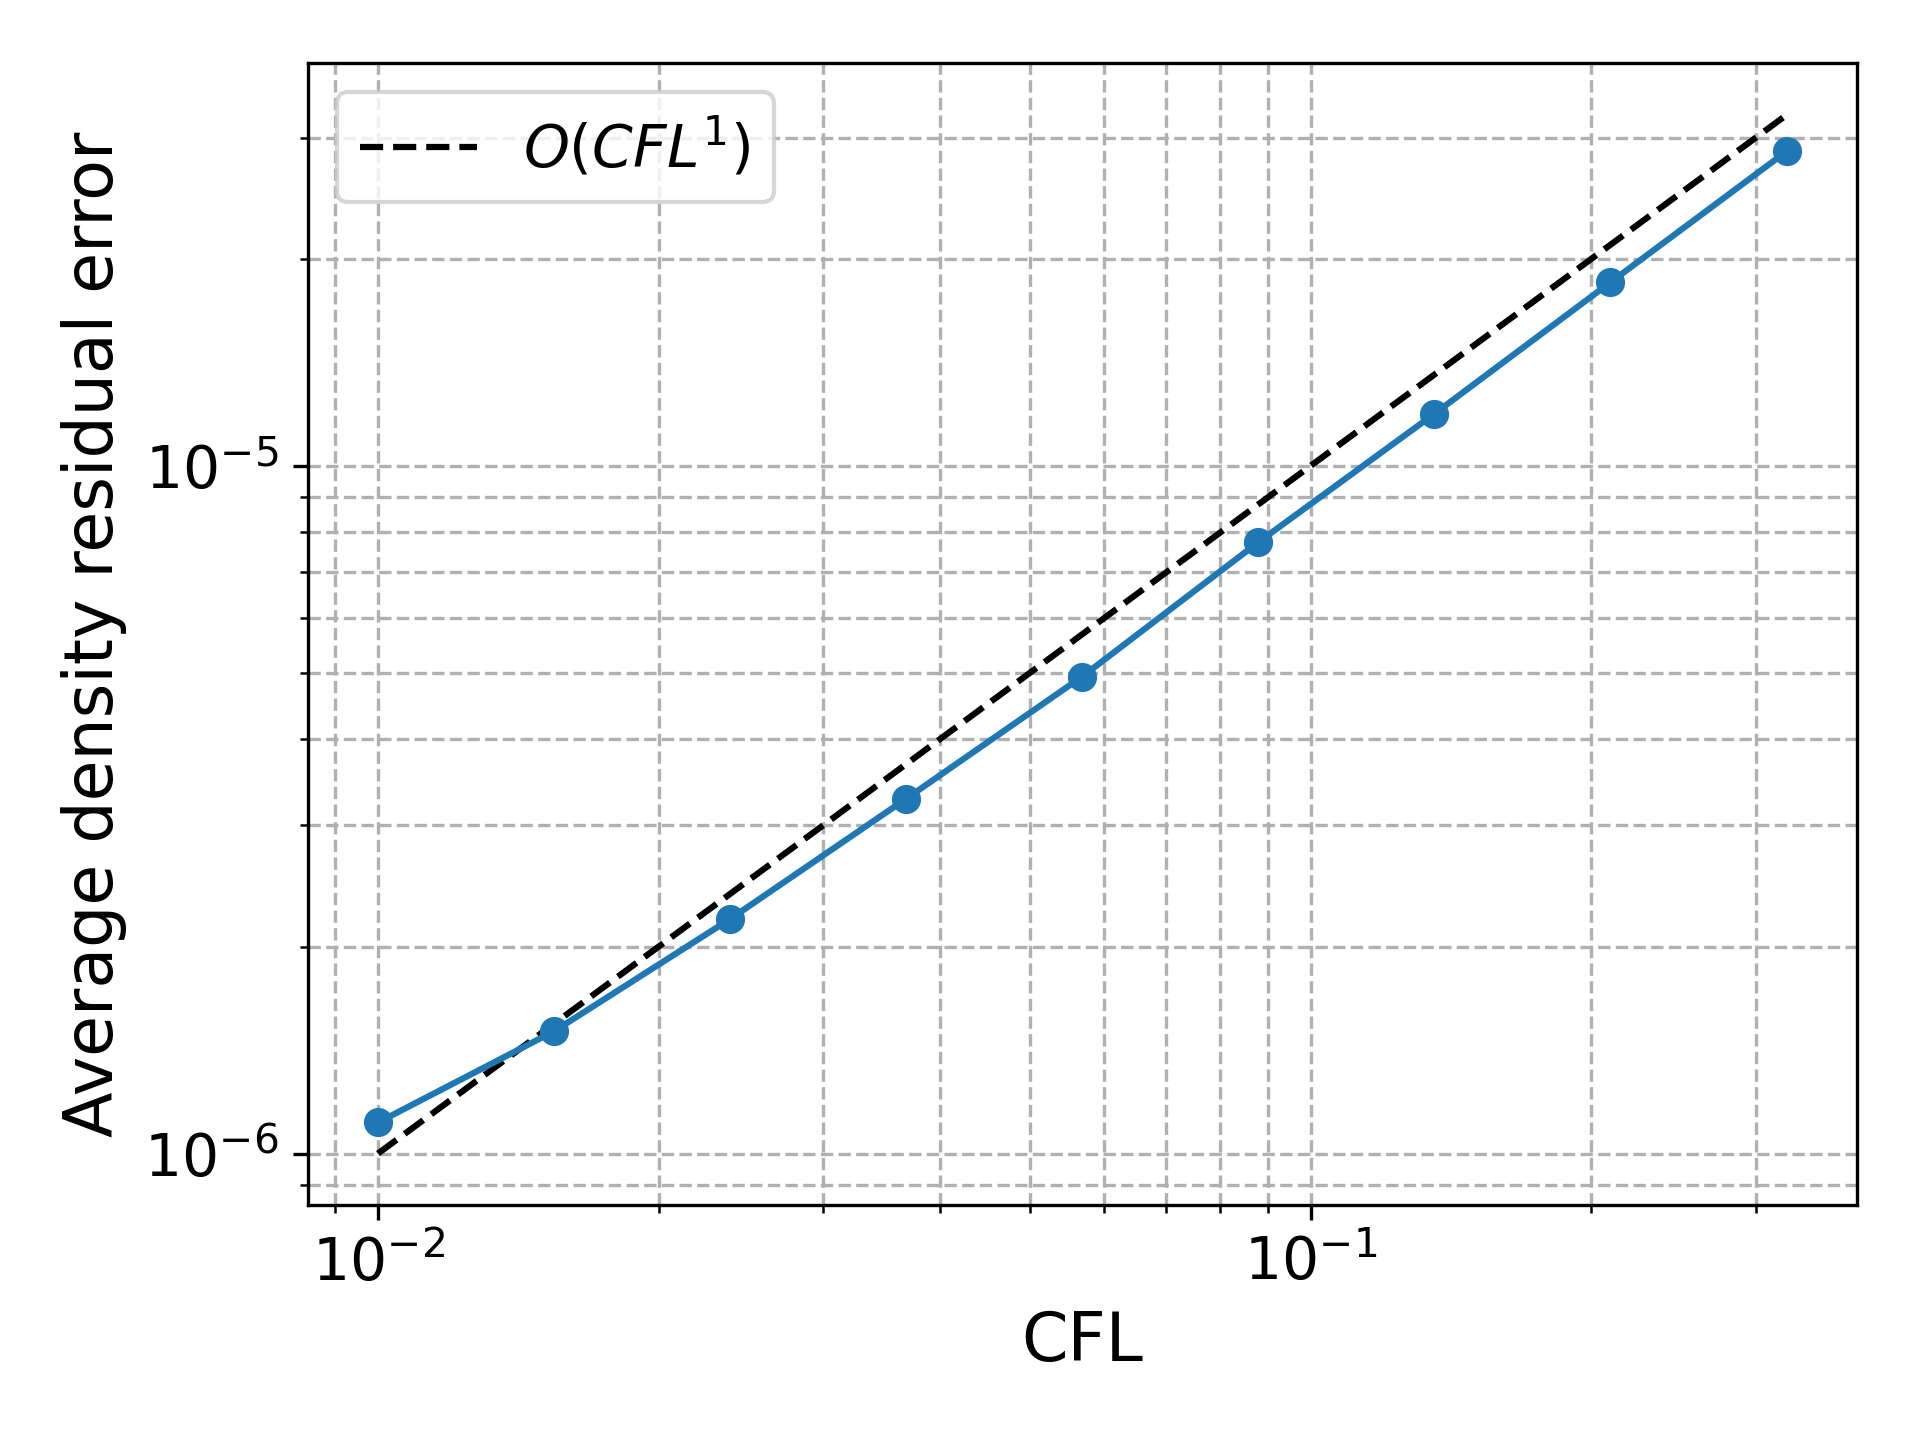
\includegraphics[width=0.99\textwidth]{figures/bump_d_avg_cfl.png}
        \caption{}
        \label{fig:bump_d_avg_cfl}
    \end{subfigure}
    \begin{subfigure}{0.49\textwidth}
        \centering
        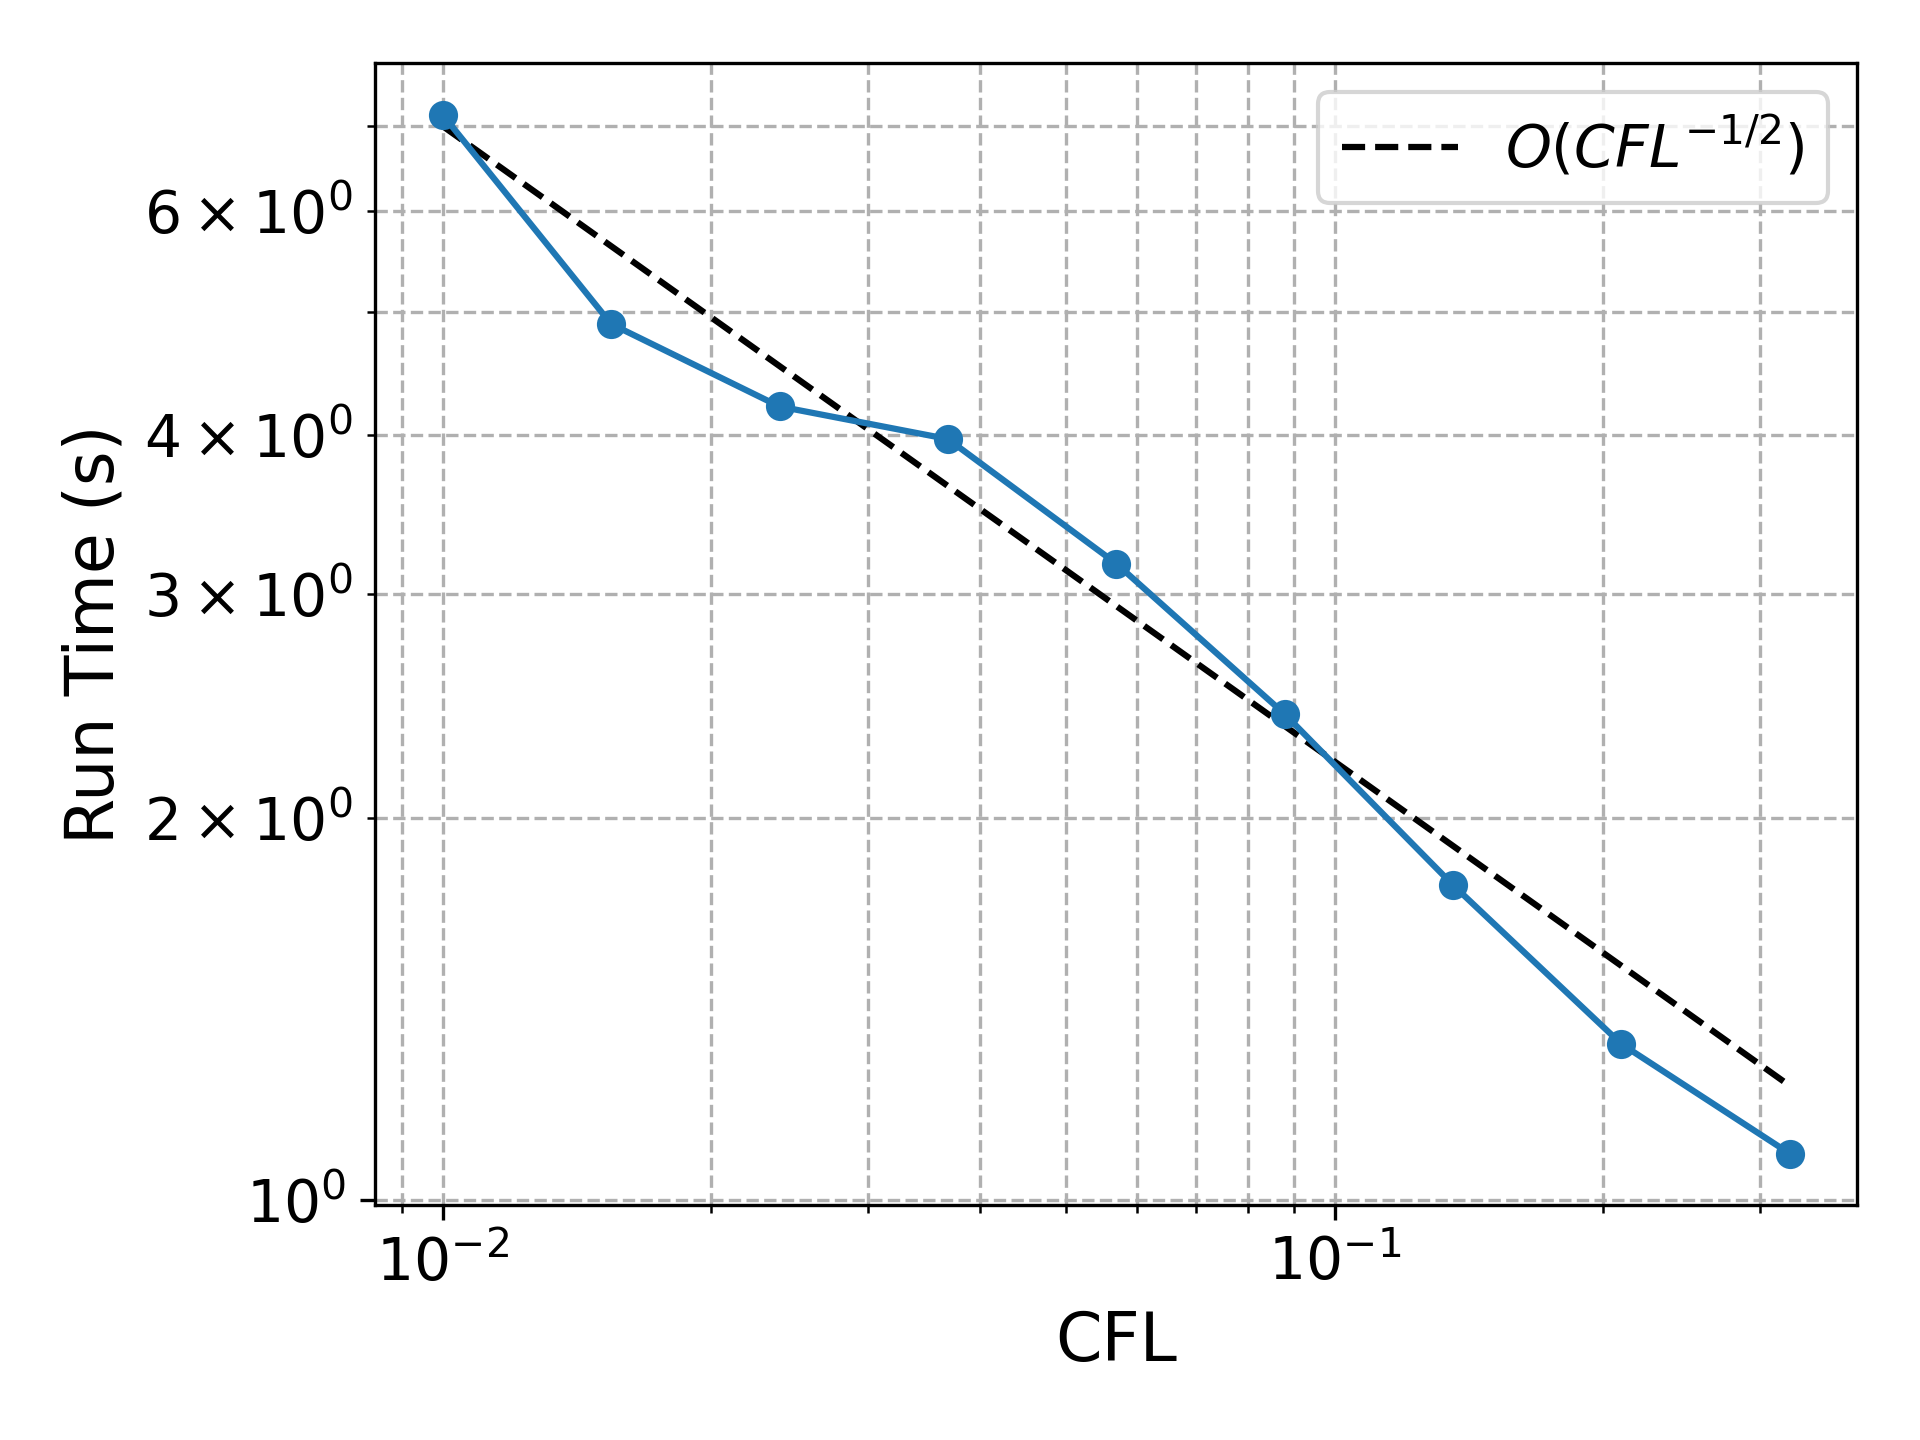
\includegraphics[width=0.99\textwidth]{figures/bump_time_cfl.png}
        \caption{}
        \label{fig:bump_time_cfl}
    \end{subfigure}
    
    \caption{Average density residual and run time against $CFL$ for the bump case where $sfac = 0.5$, $ni = 53$.}
\end{figure}

\begin{figure}[H]
    \centering
    \begin{subfigure}{0.49\textwidth}
        \centering
        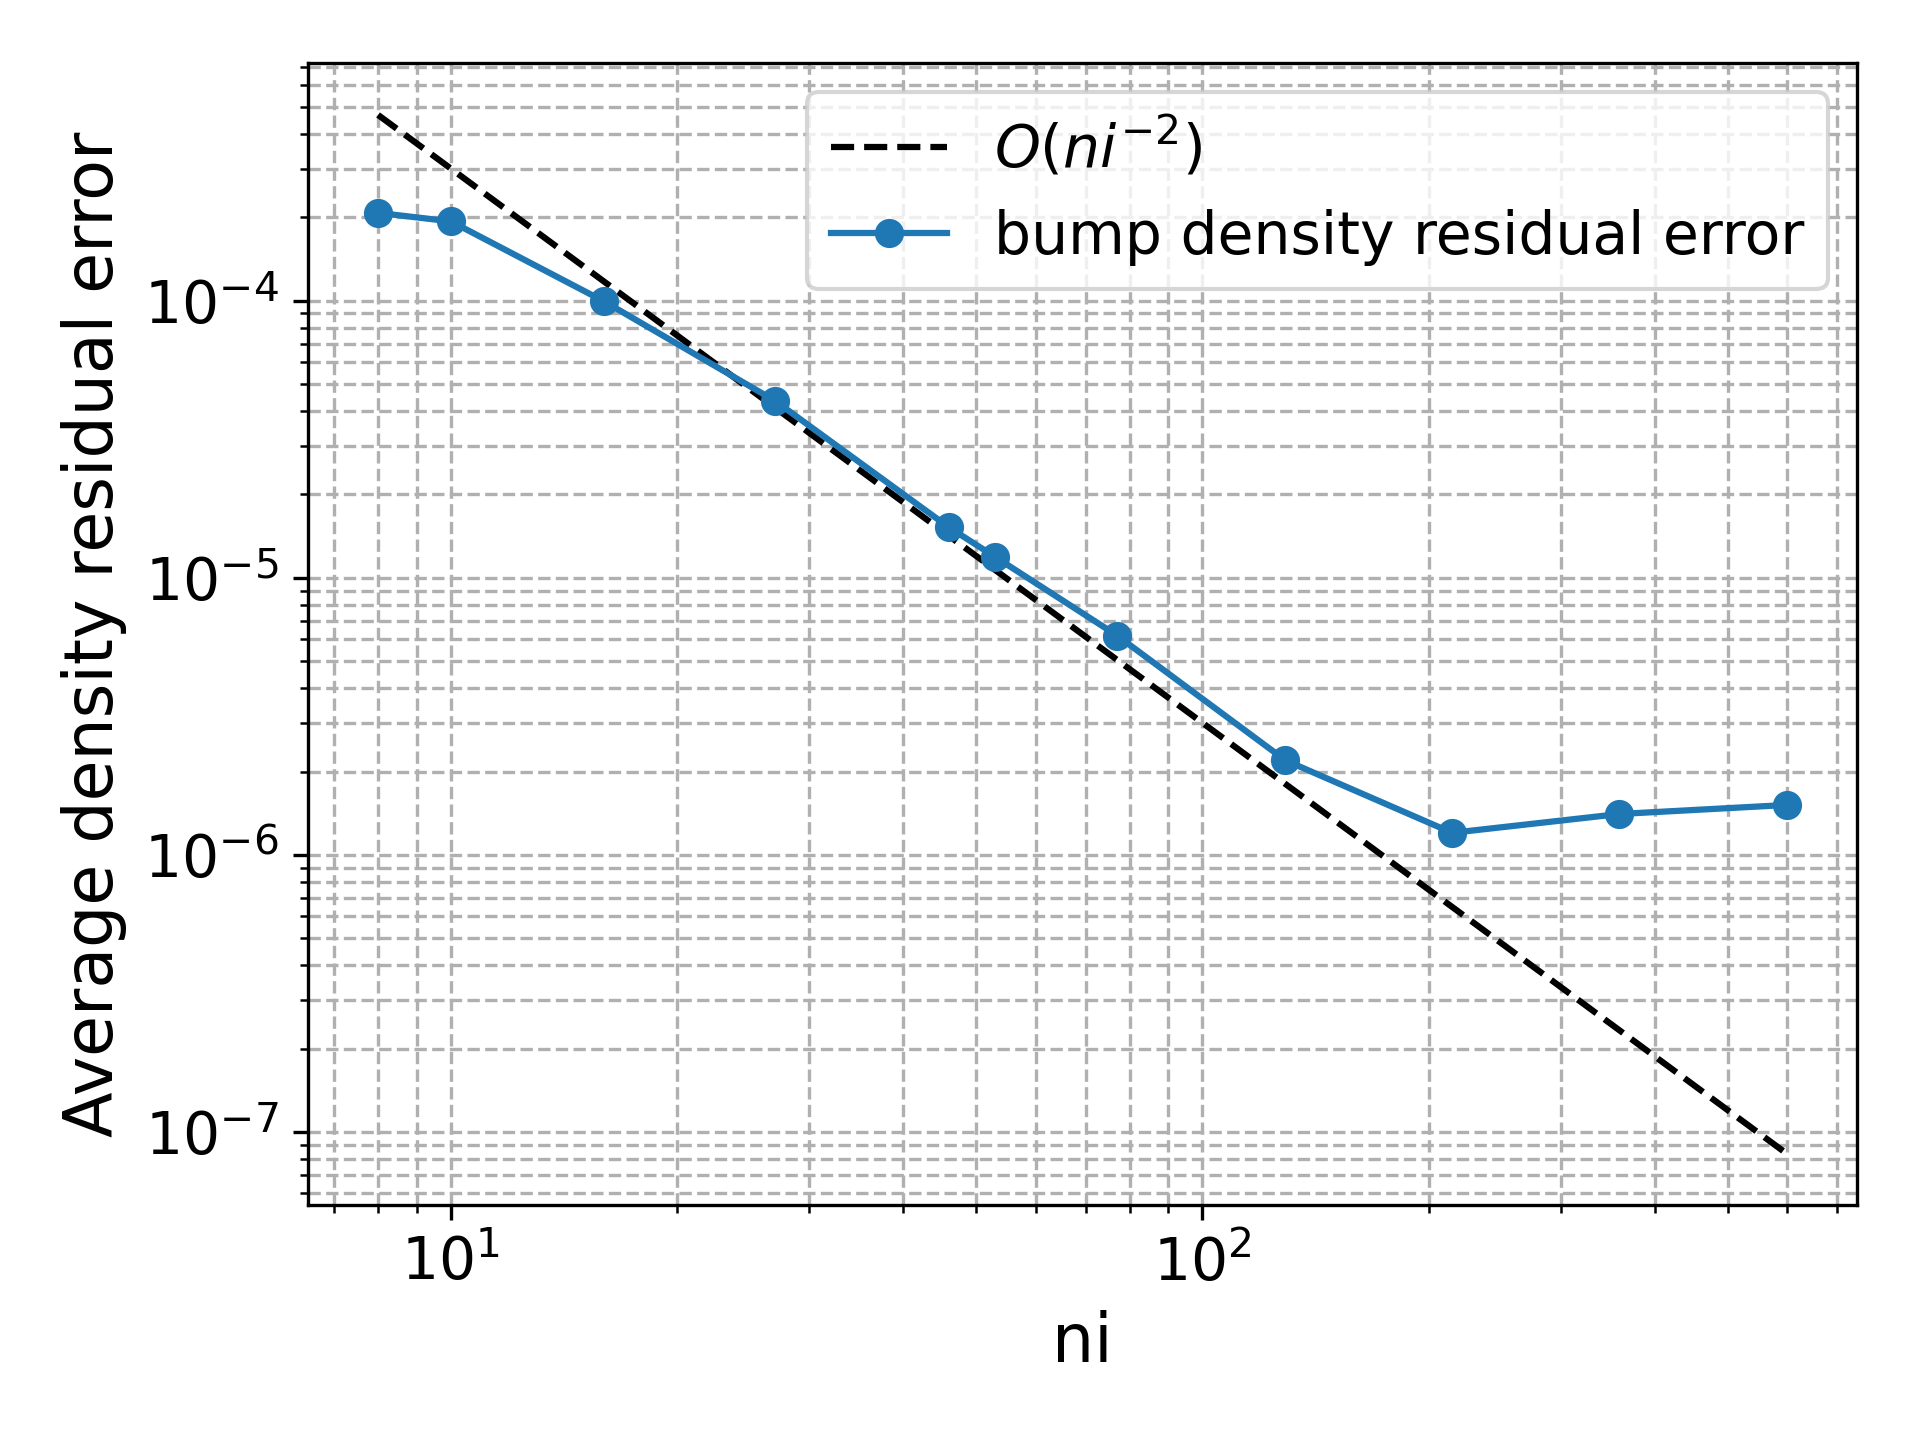
\includegraphics[width=0.99\textwidth]{figures/bump_d_avg_ni.png}
        \caption{}
        \label{fig:bump_d_avg_ni}
    \end{subfigure}
    \begin{subfigure}{0.49\textwidth}
        \centering
        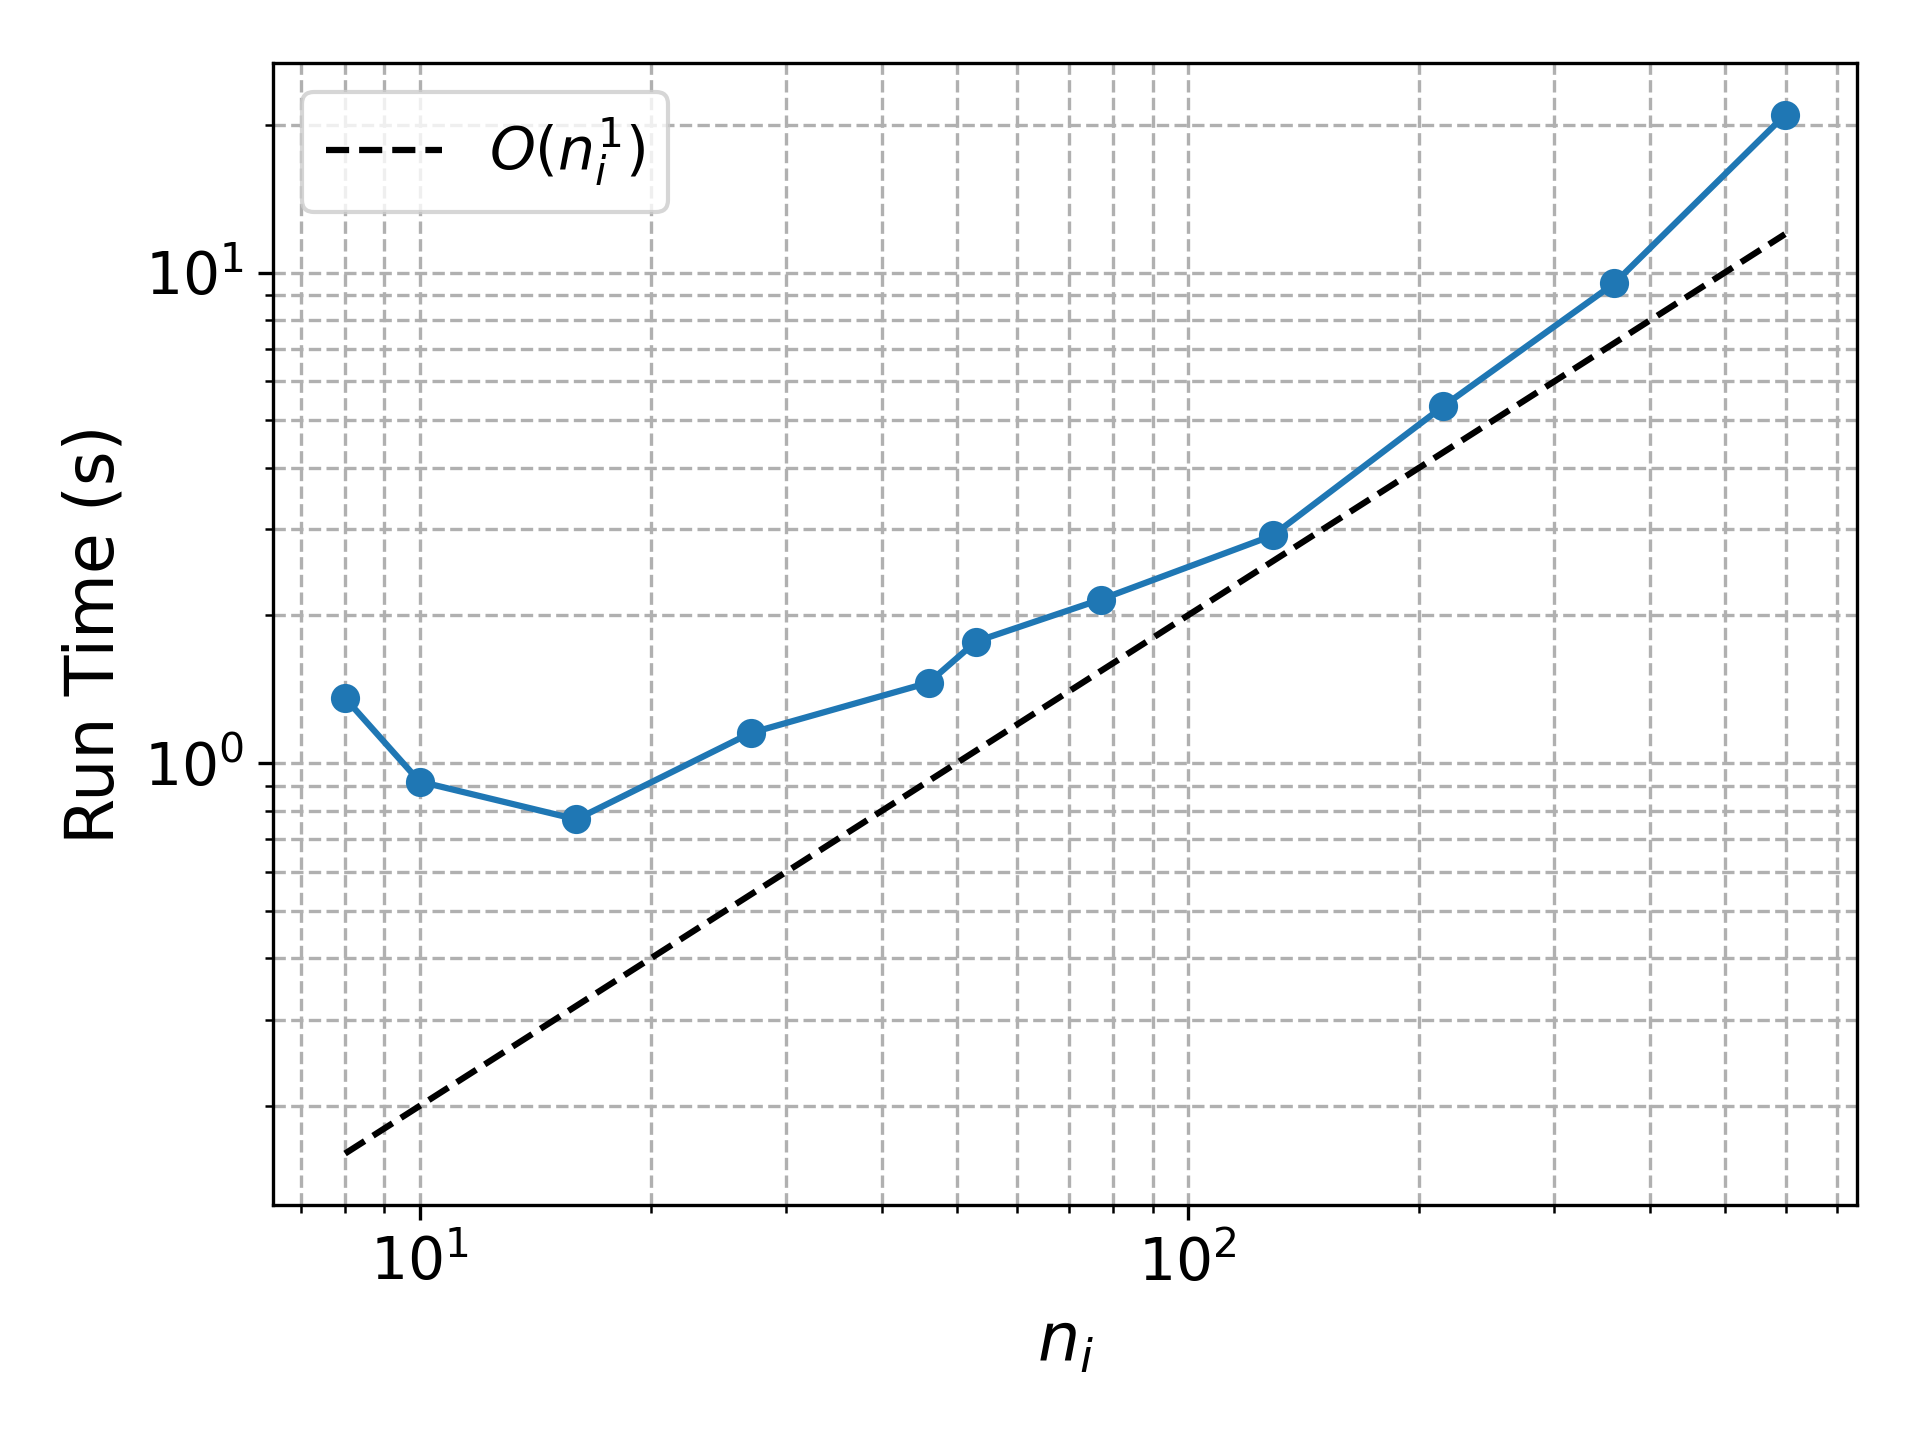
\includegraphics[width=0.99\textwidth]{figures/bump_time_ni.png}
        \caption{}
        \label{fig:bump_time_ni}
    \end{subfigure}
    \caption{Average density residual and run time against $n_i$ for the bump case where $sfac = 0.5$, $sfac = 0.1357$.}
\end{figure}

\begin{figure}
    \centering
    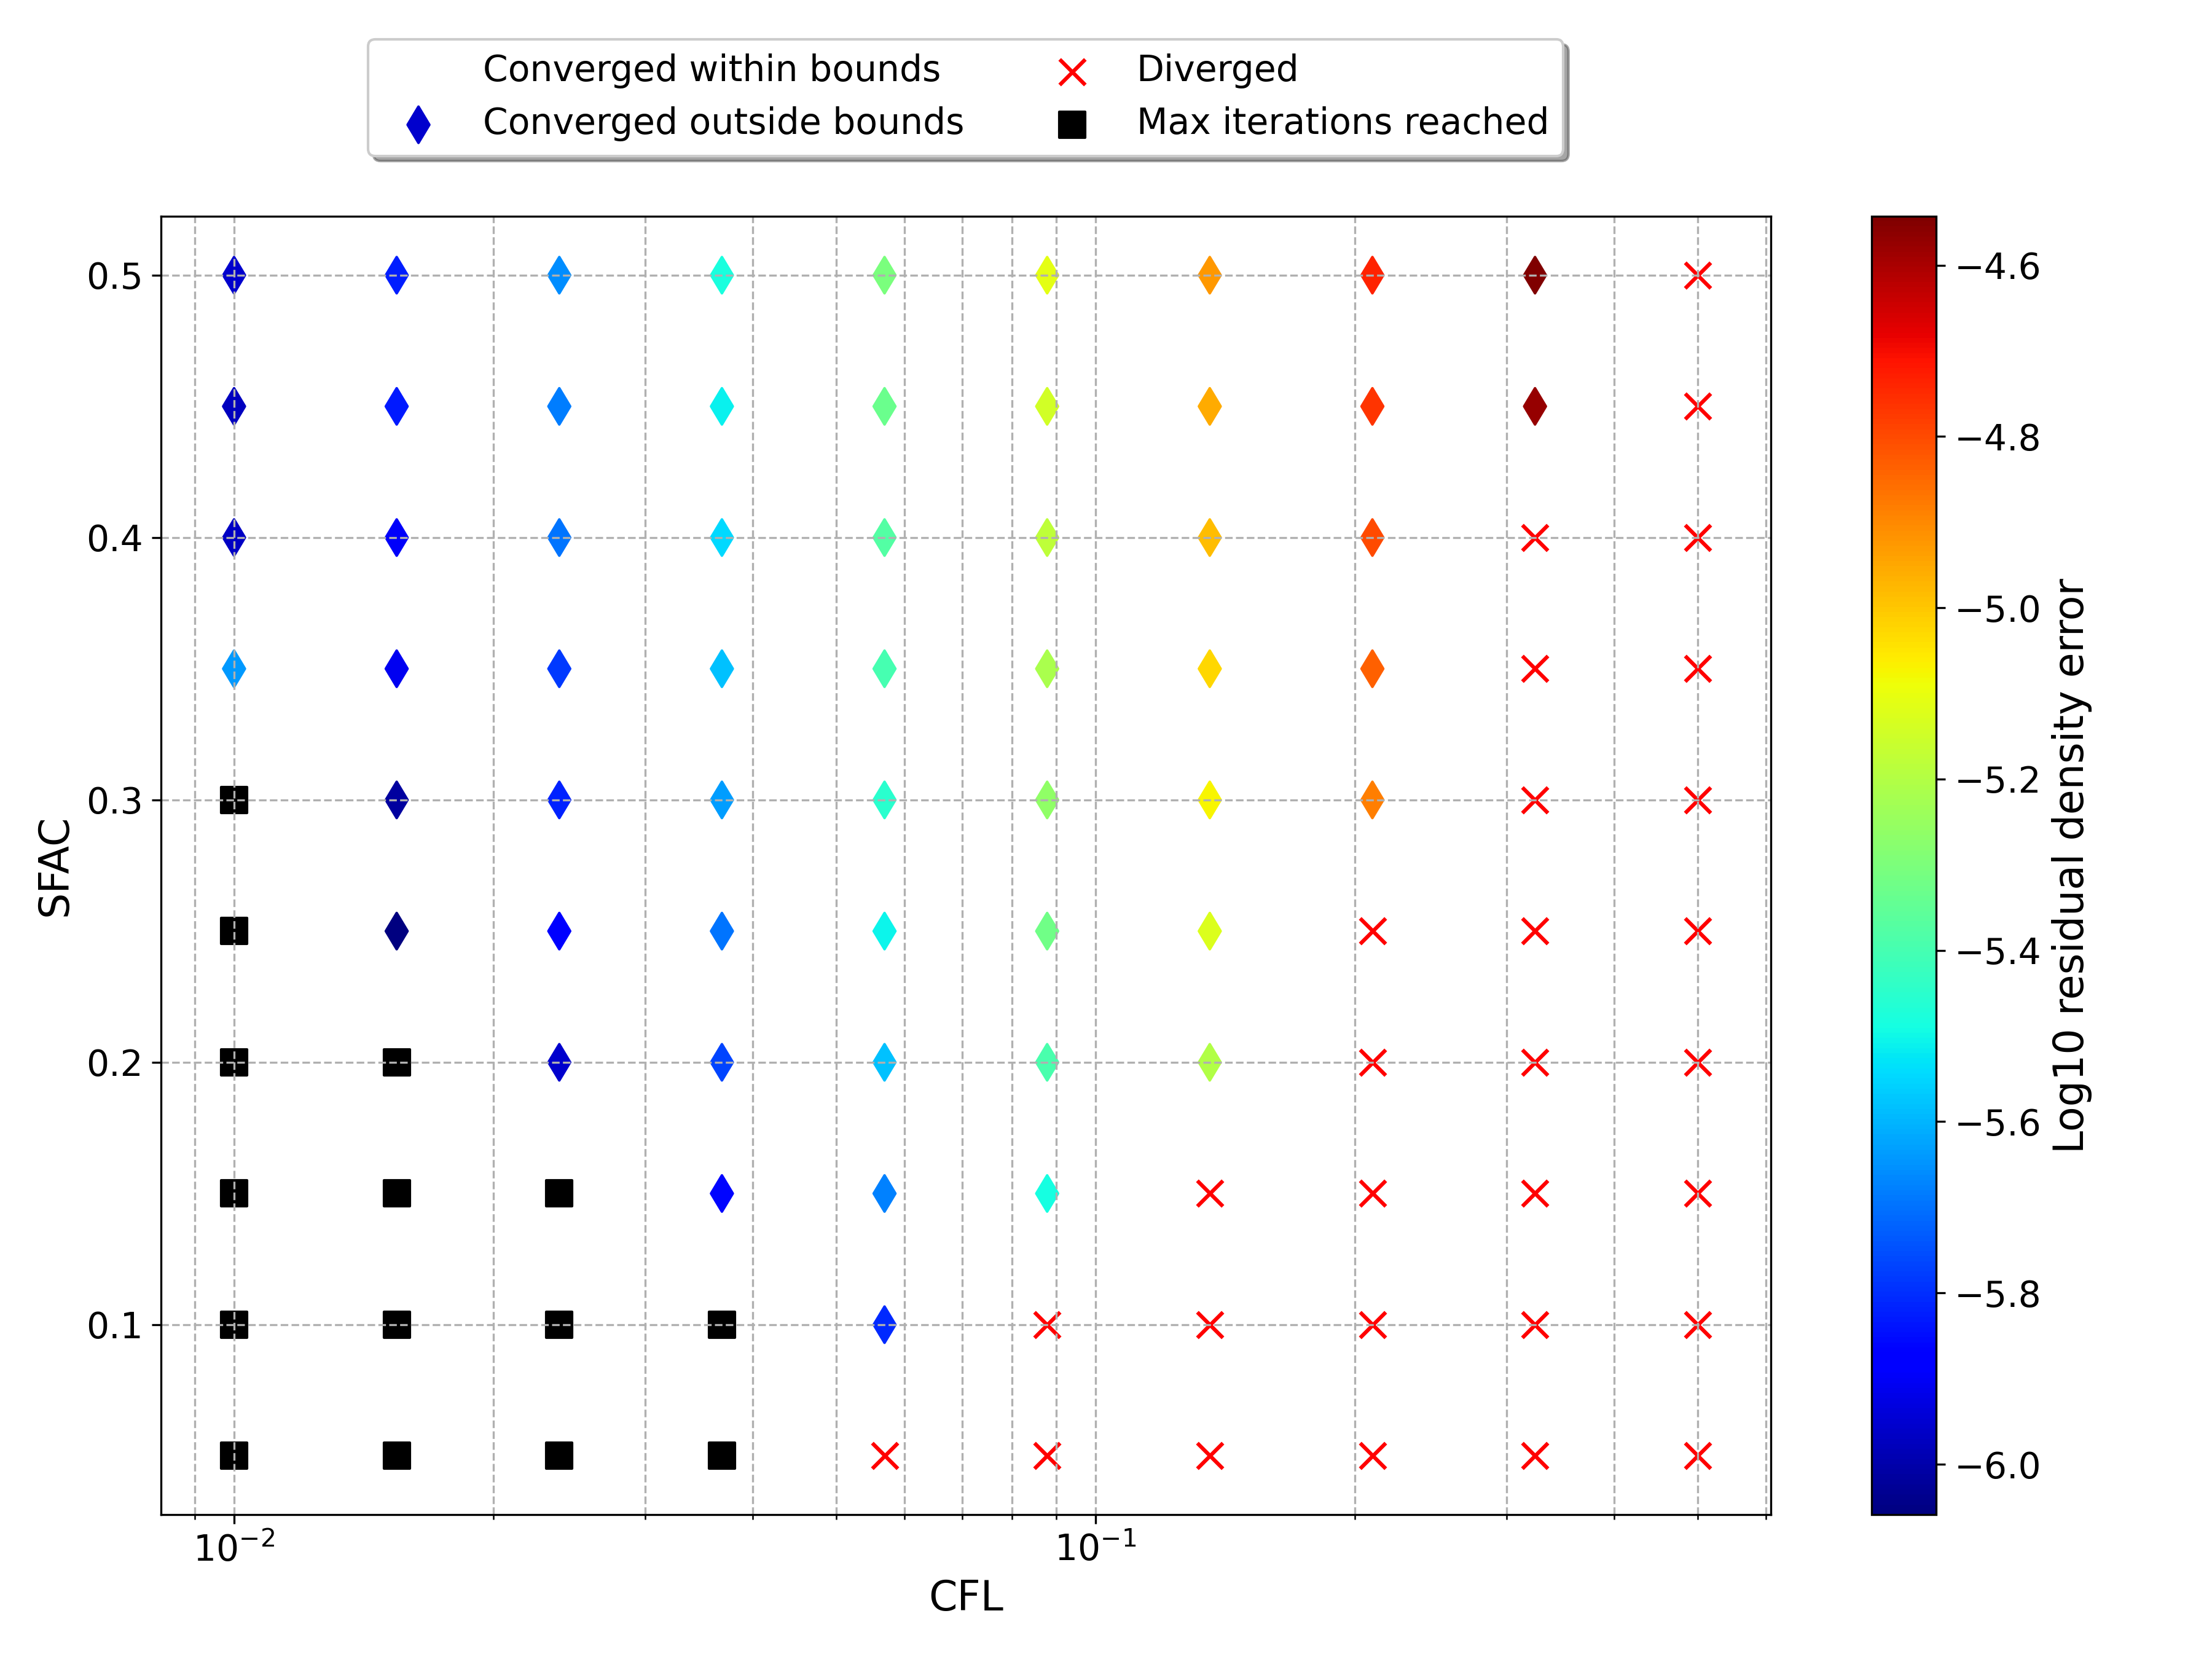
\includegraphics[width=0.8\textwidth]{figures/bump_cfl_sfac_residual.png}
    \caption{Scatter plot showing variation in residual error for different CFL and sfac values.}
    \label{fig:bump_cfl_sfac_residual}
\end{figure}

\begin{figure}[H]
    \centering
    \centering
    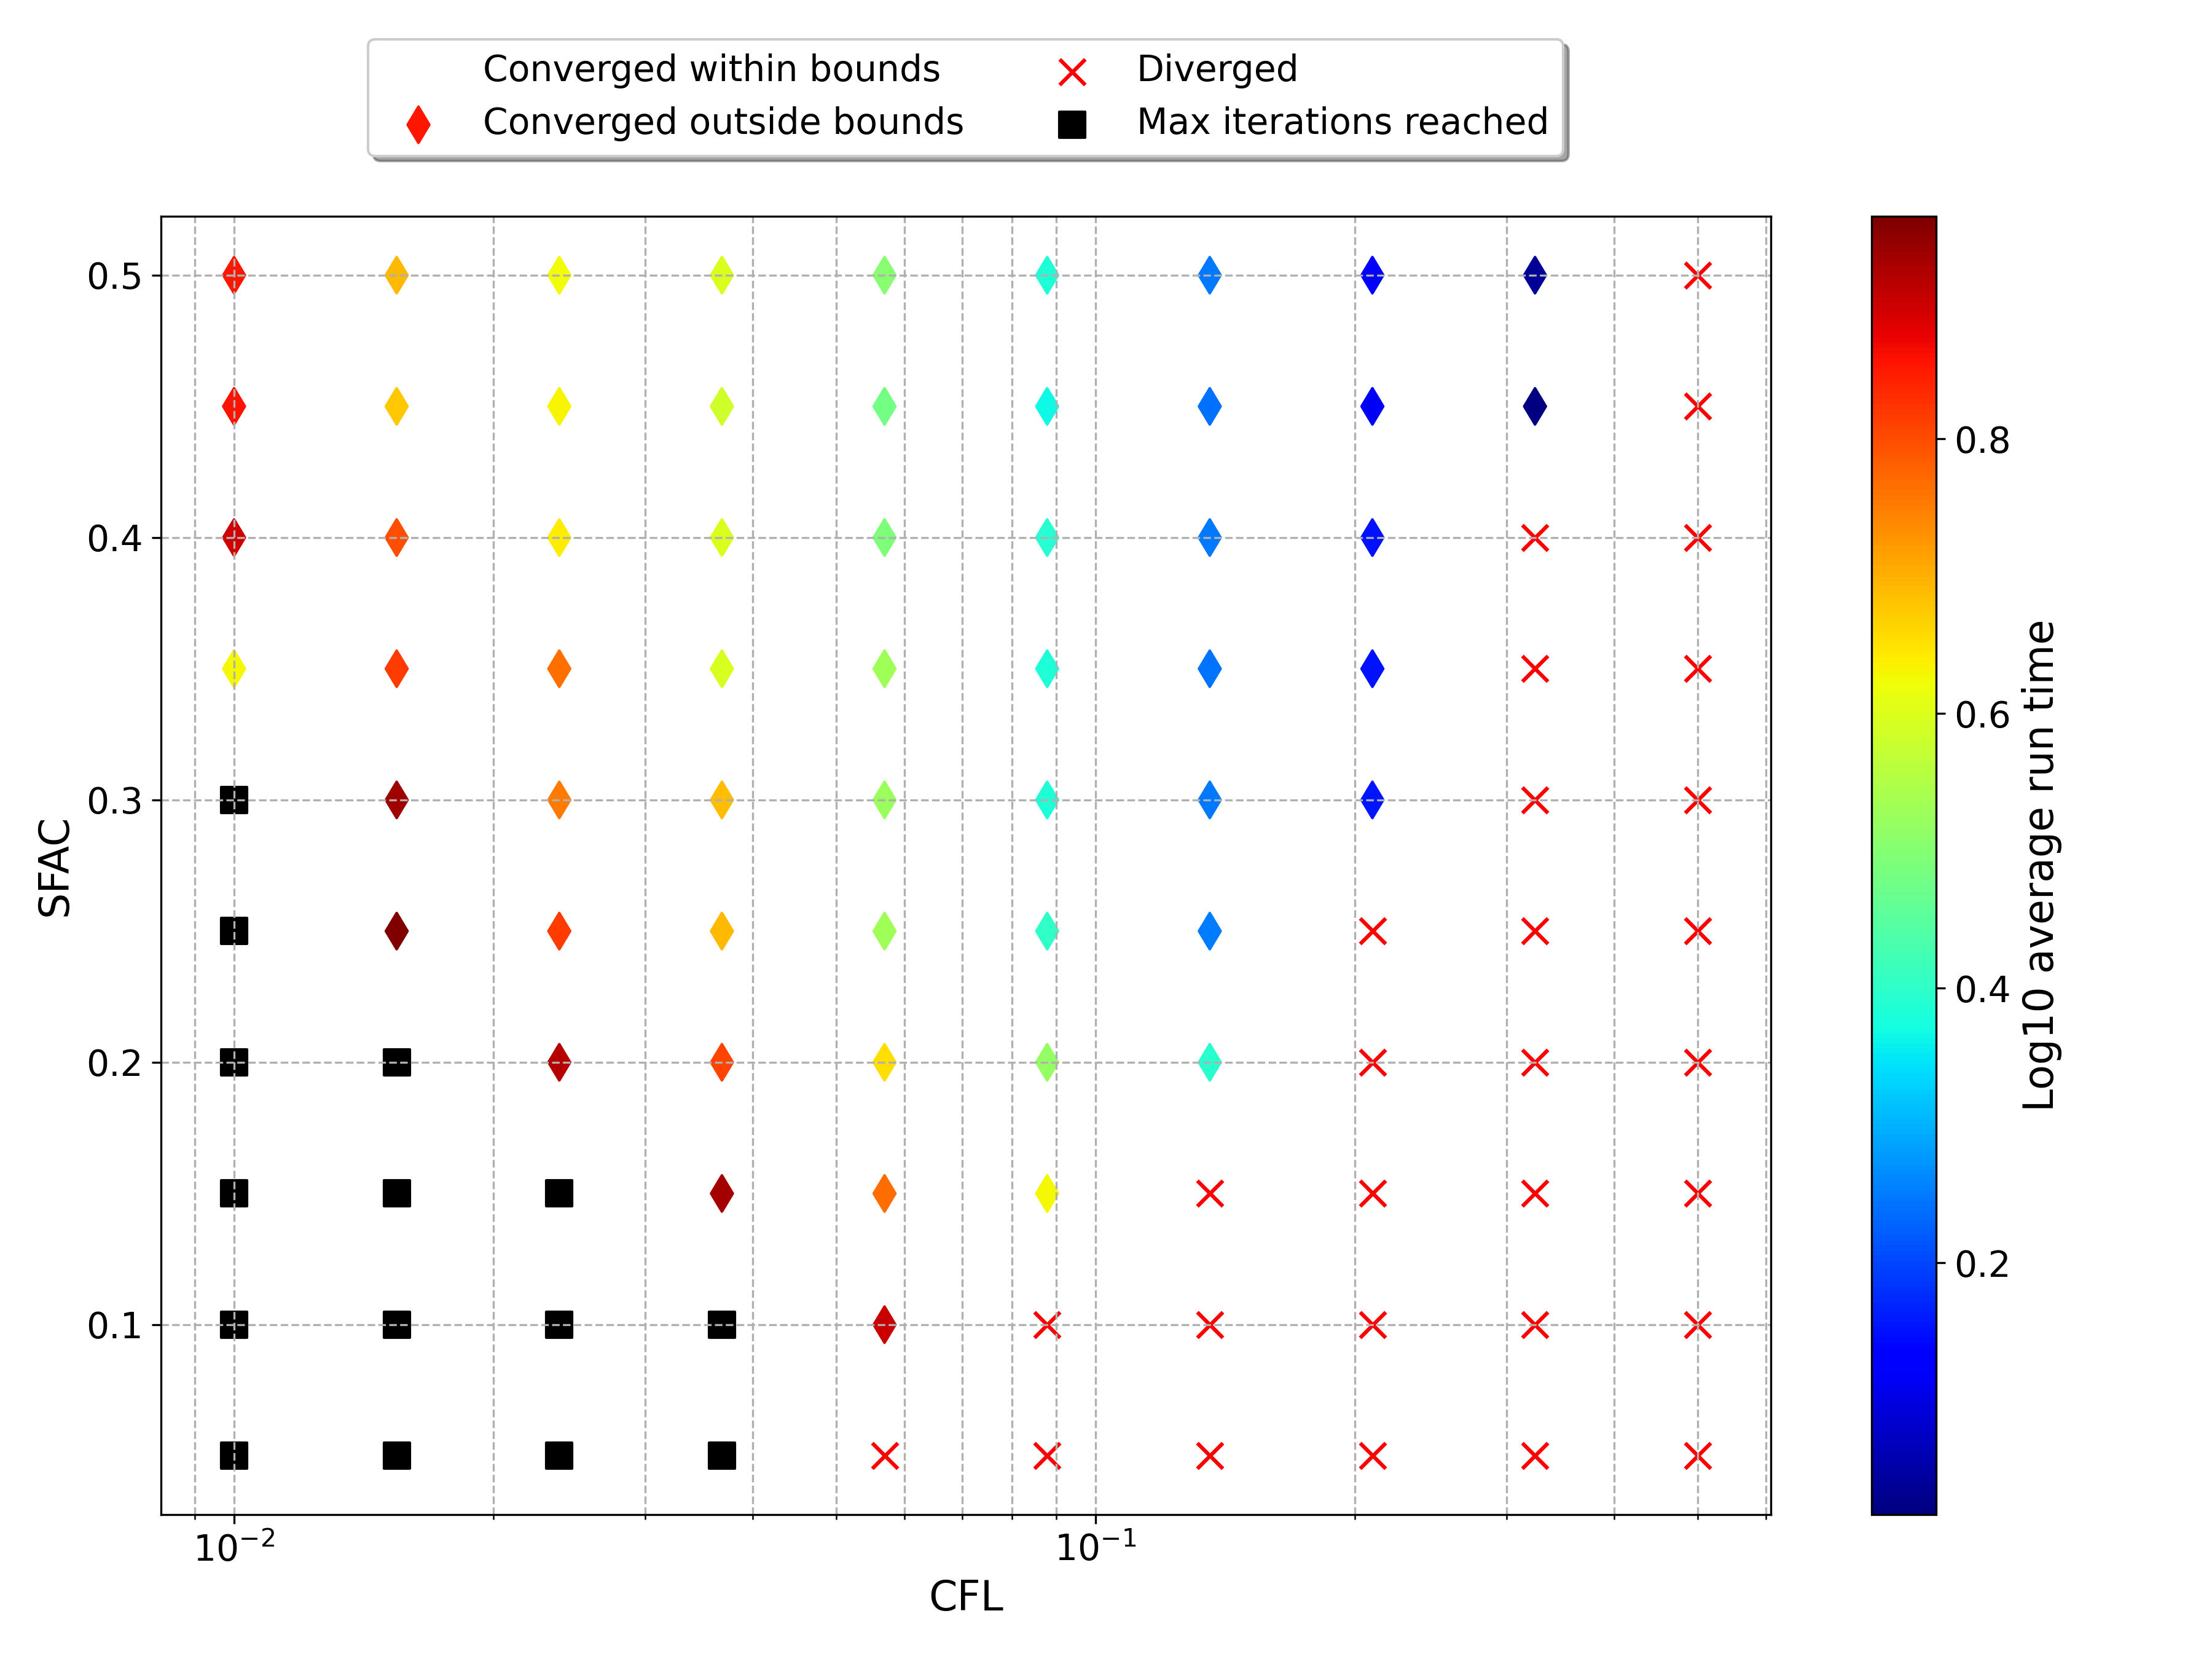
\includegraphics[width=0.8\textwidth]{figures/bump_cfl_sfac_time.png}
    \caption{Scatter plot showing variation in run time for different CFL and sfac values.}
    \label{fig:bump_cfl_sfac_time}
\end{figure}

\subsection{Bend test case}

\begin{figure}[H]
    \centering
    \begin{subfigure}{0.99\textwidth}
        \centering
        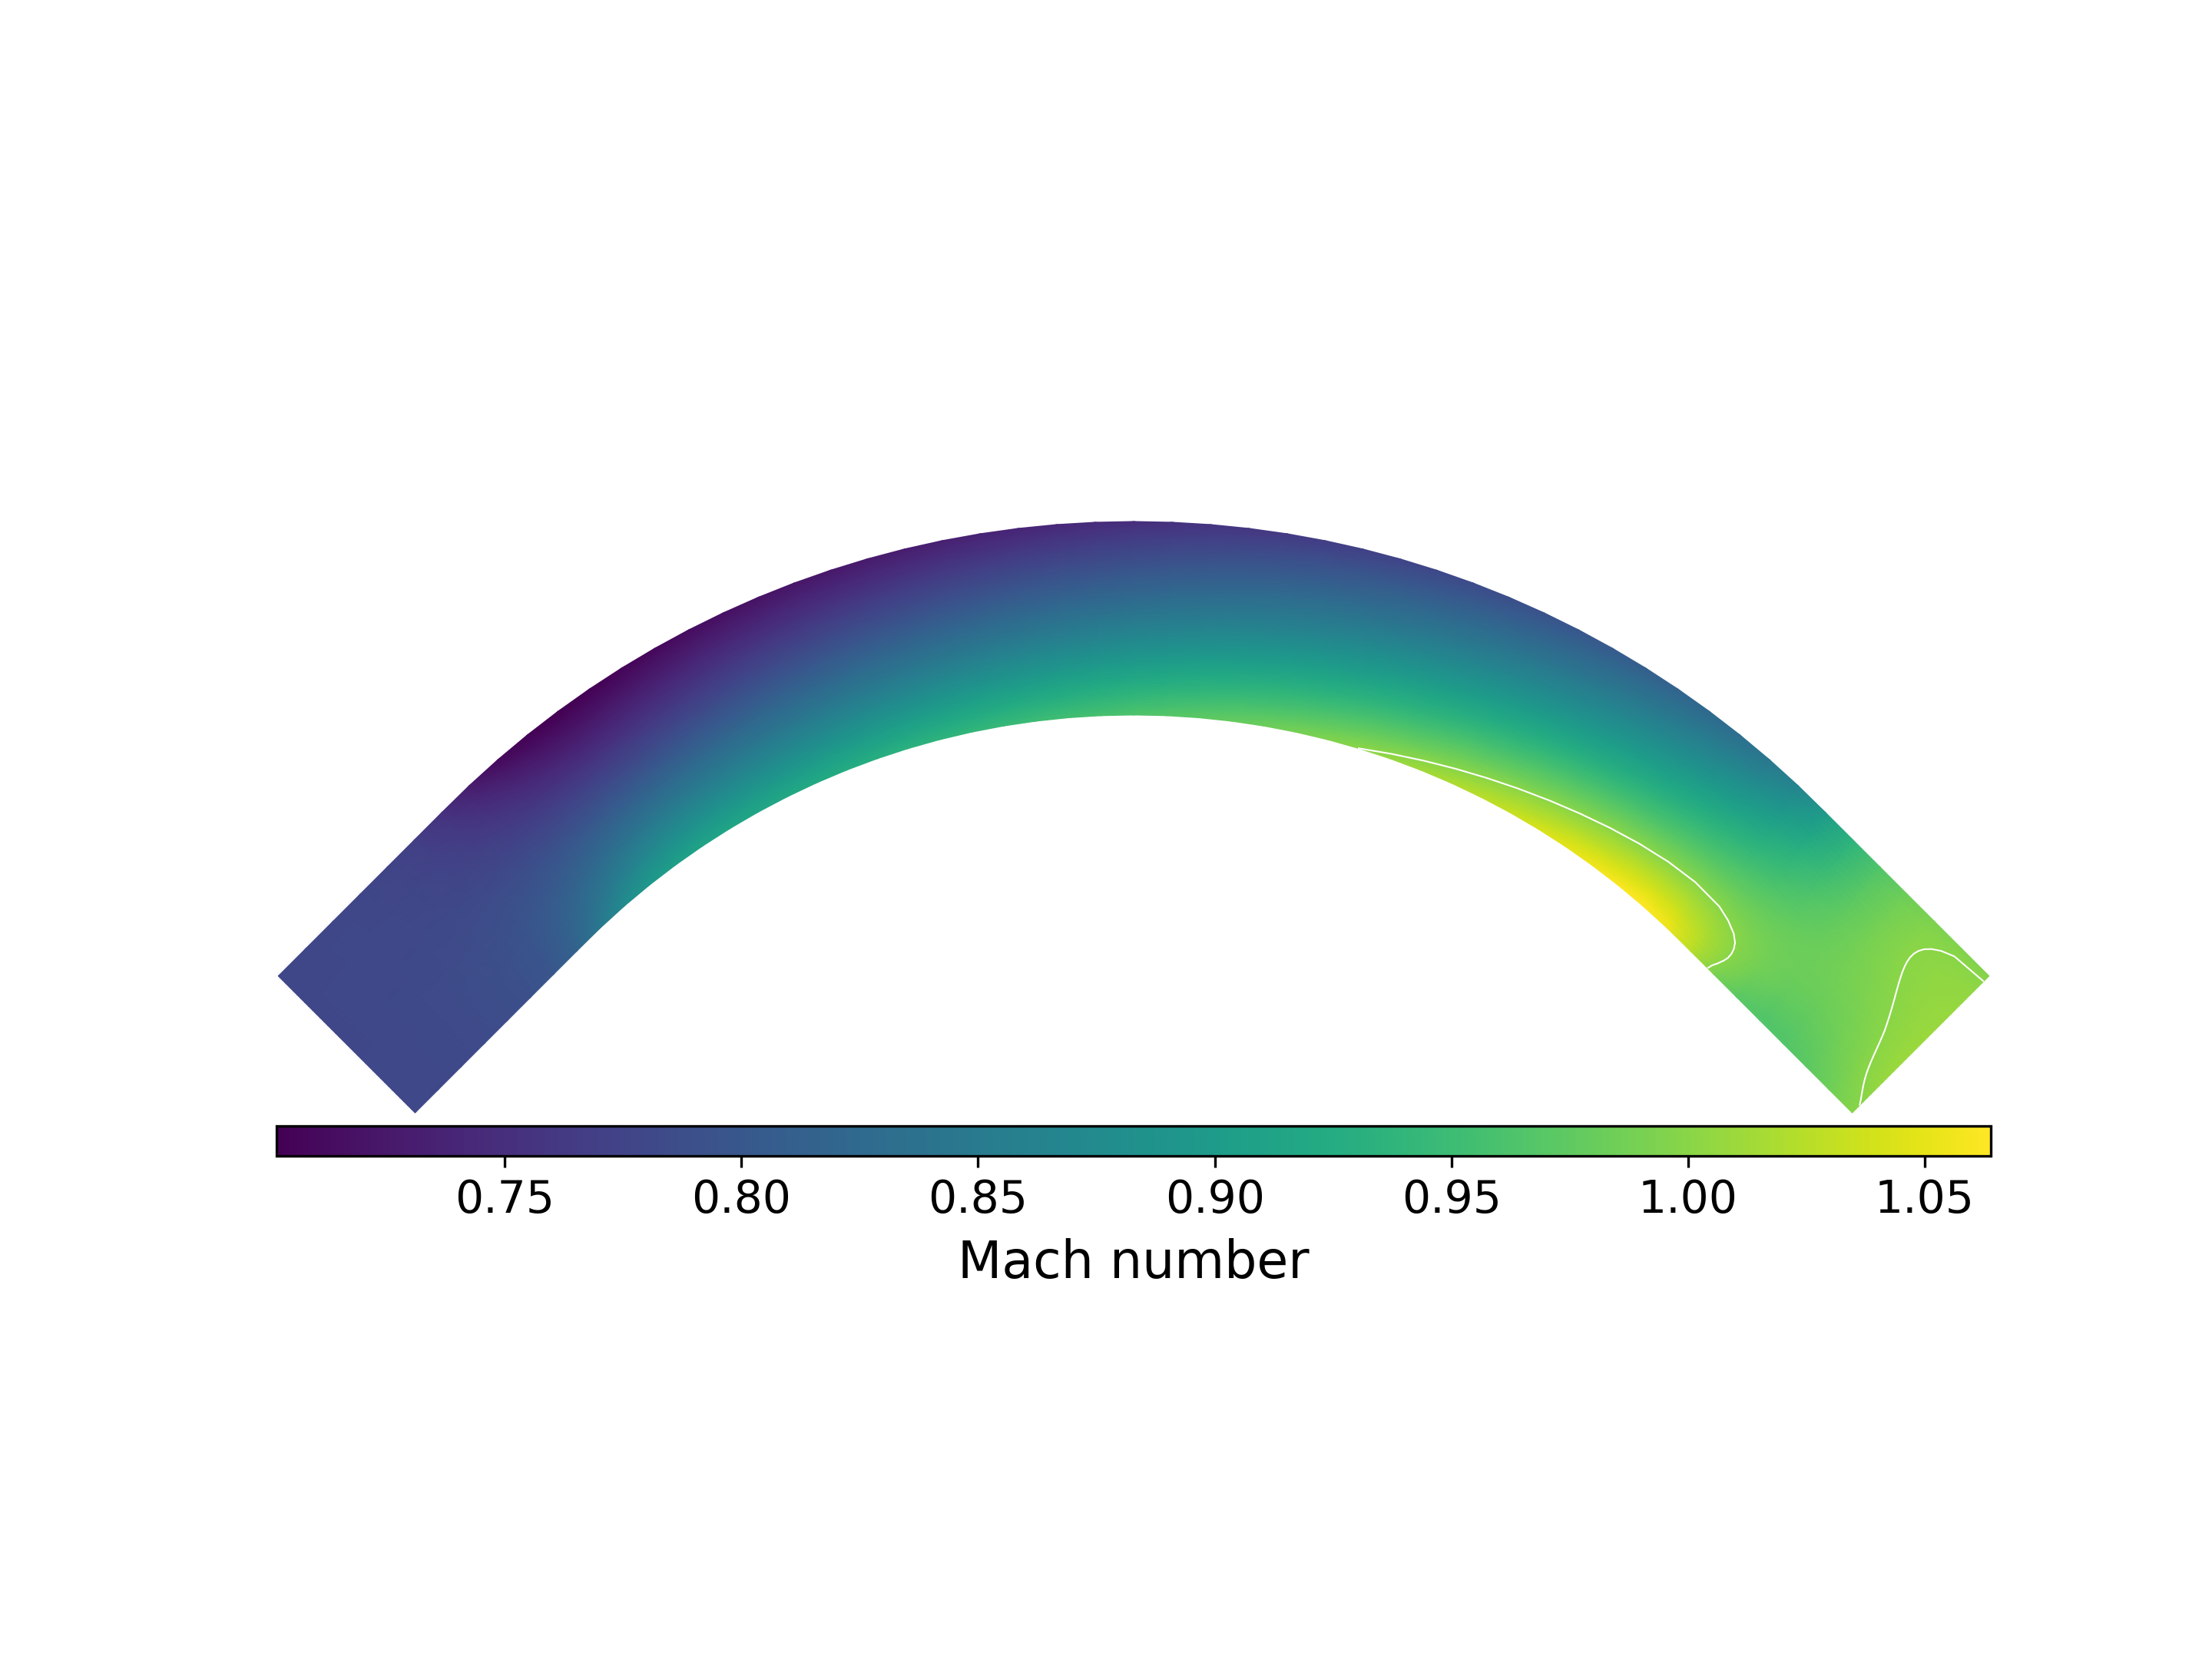
\includegraphics[width=0.7\textwidth]{figures/bend_mach.png}
        \caption{}
        \label{fig:bend_mach}
    \end{subfigure}
    \begin{subfigure}{0.99\textwidth}
        \centering
        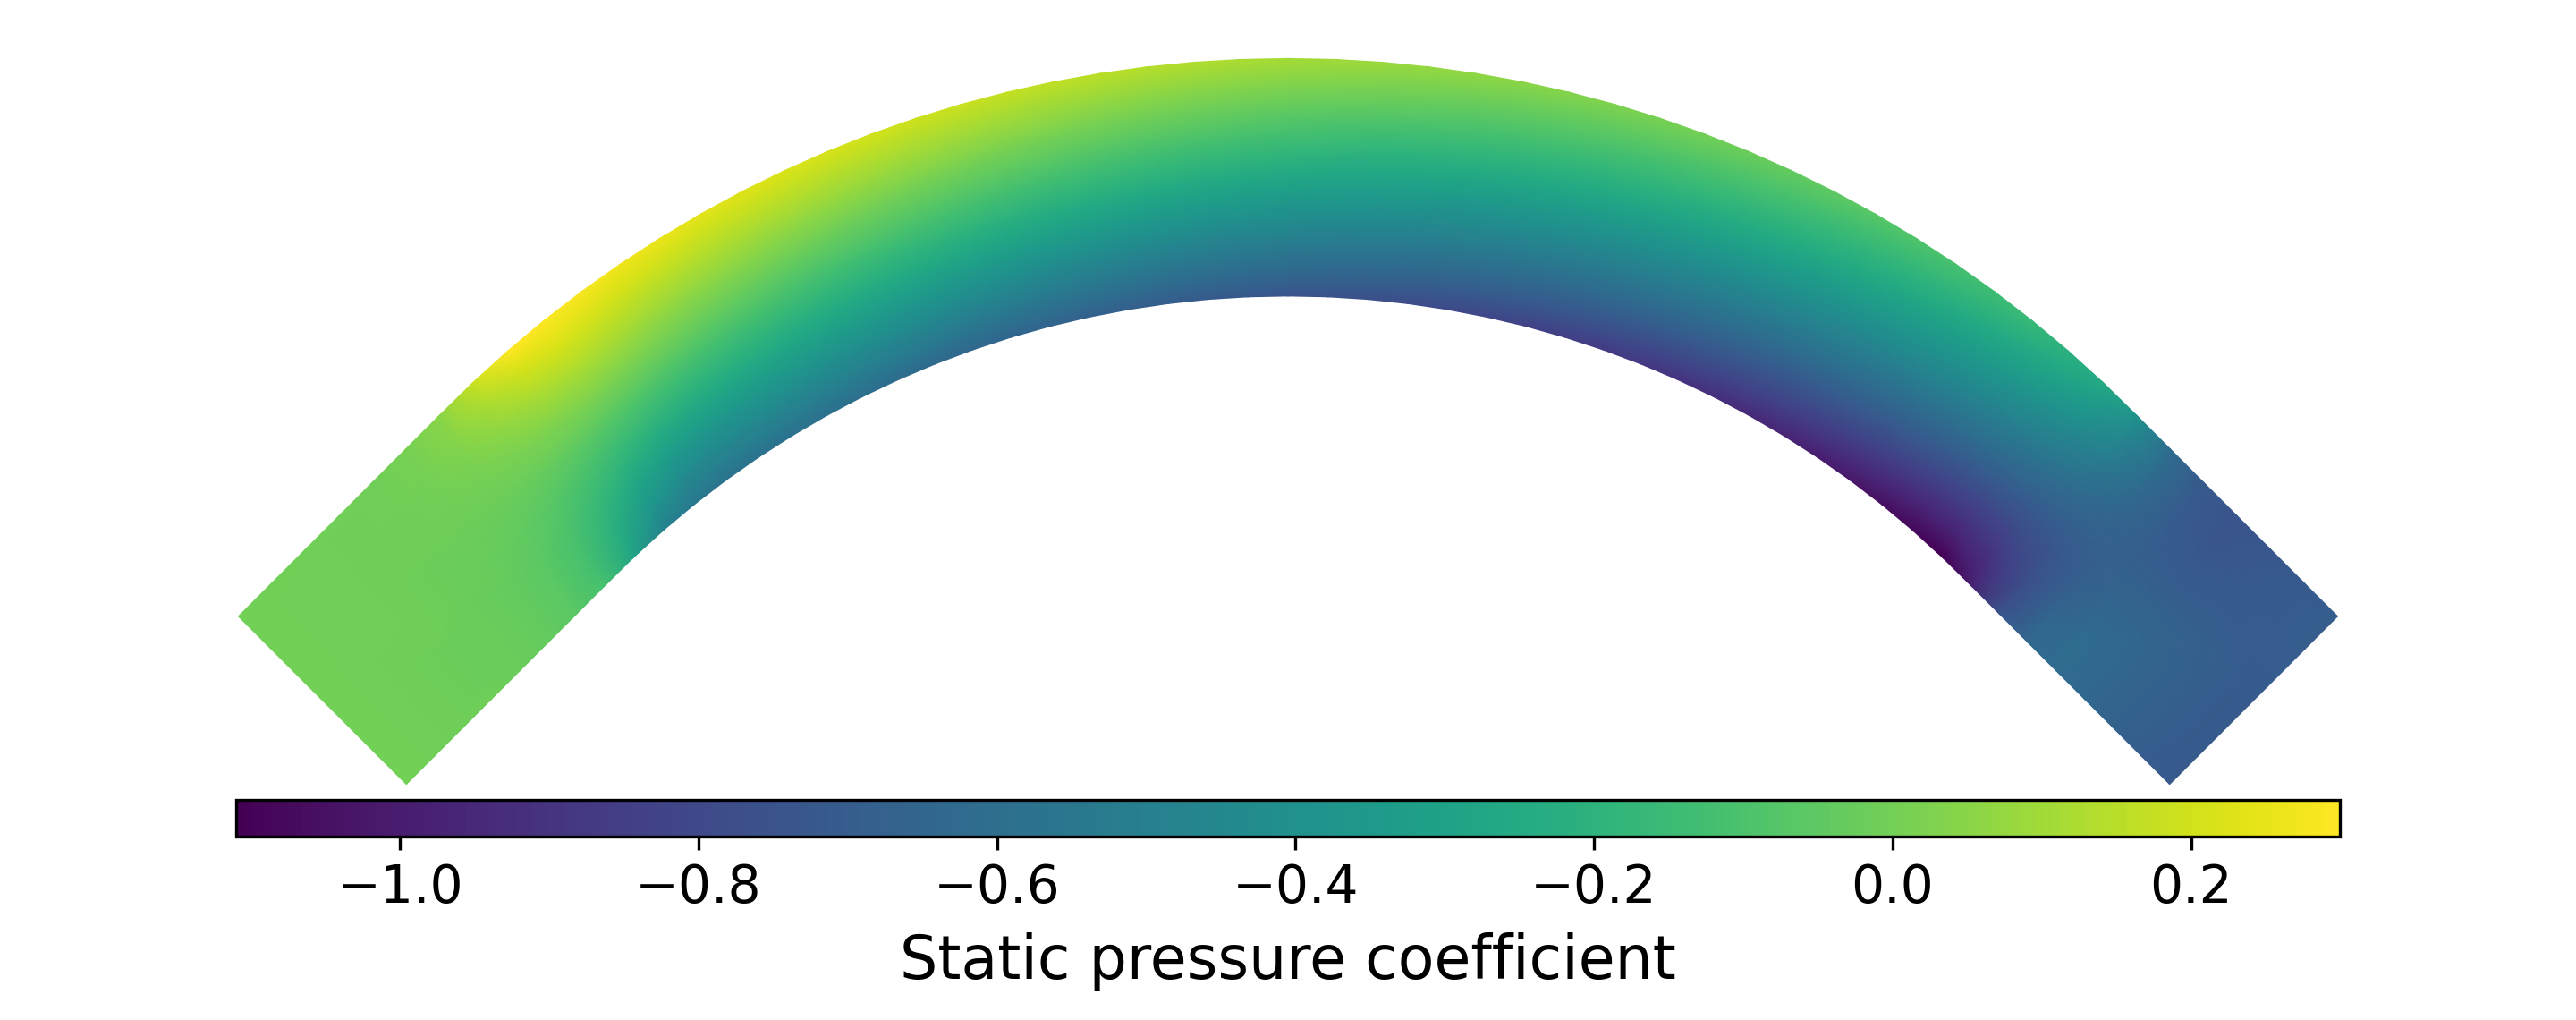
\includegraphics[width=0.7\textwidth]{figures/bend_cp.png}
        \caption{}
        \label{fig:bend_cp}
    \end{subfigure}
    \caption{Bend test case results $CFL = 0.05$, $sfac = 0.1$, $n_i = 53$, $n_j = 37$}
\end{figure}

\begin{figure}[H]
    \centering
    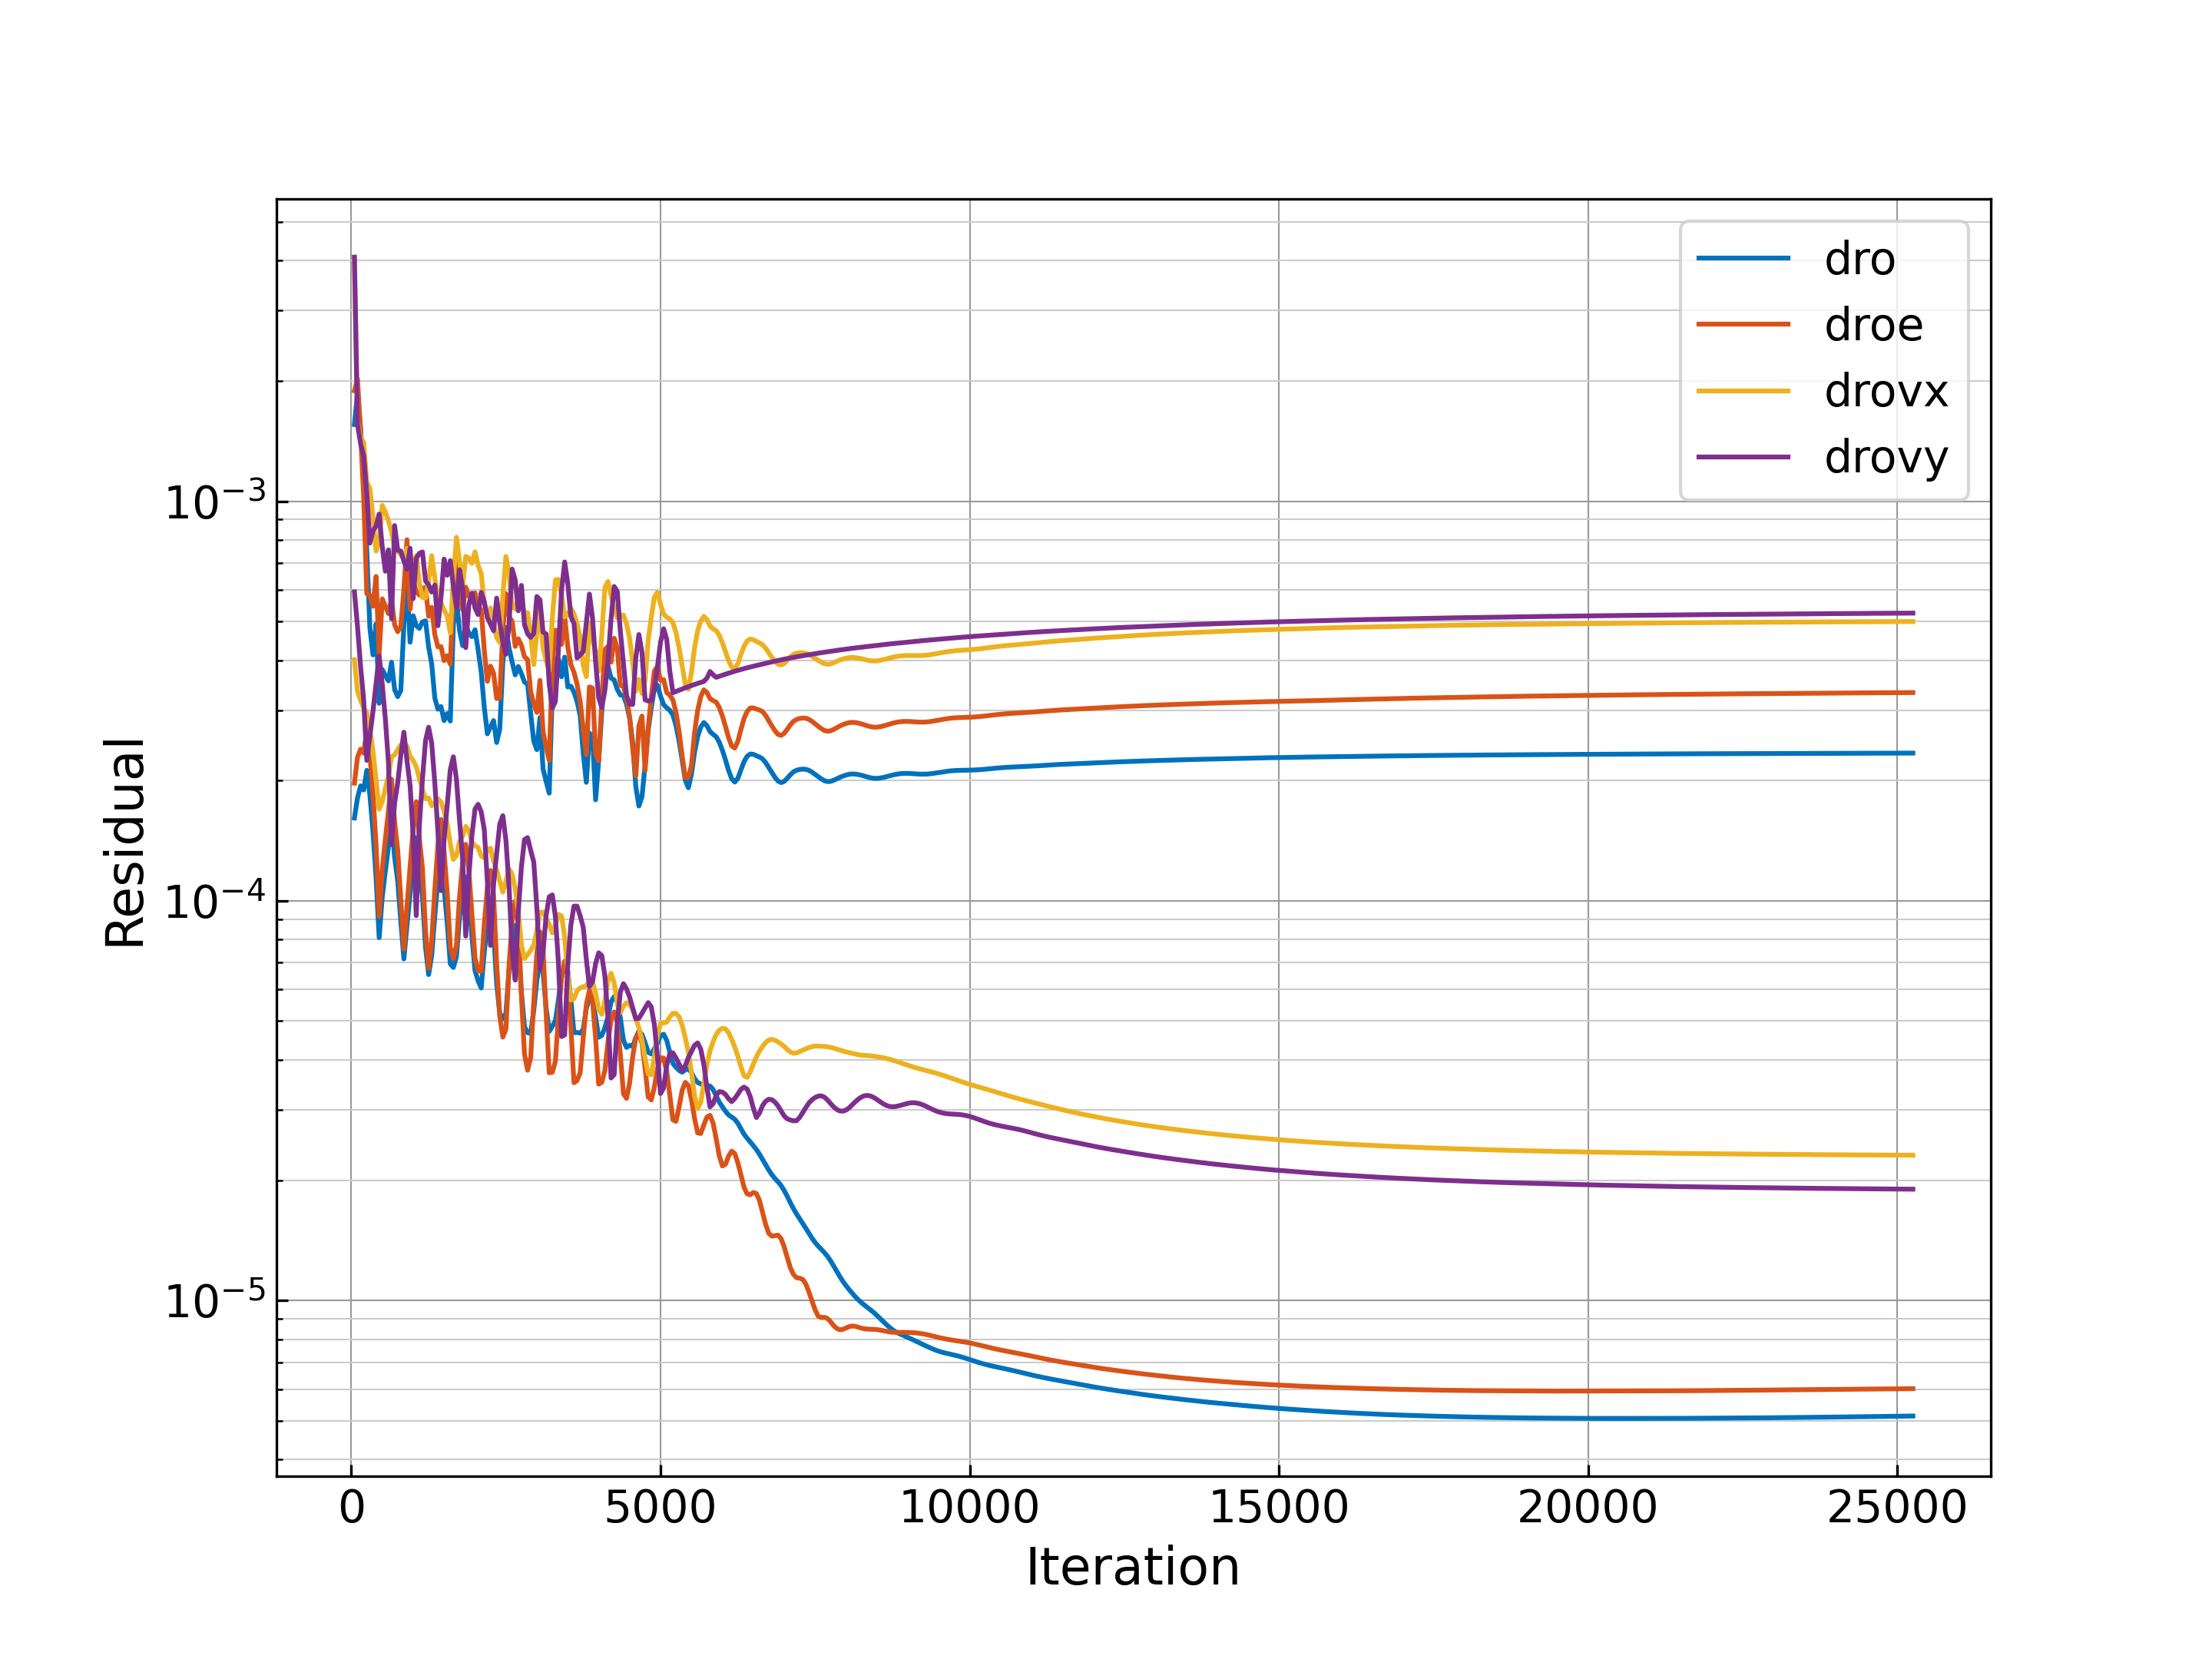
\includegraphics[width=0.8\textwidth]{figures/bend_conv.png}
    \caption{Convergence history of primary flow variables for the bend case}
    \label{fig:bend_conv}
\end{figure}

\begin{figure}
    \centering
    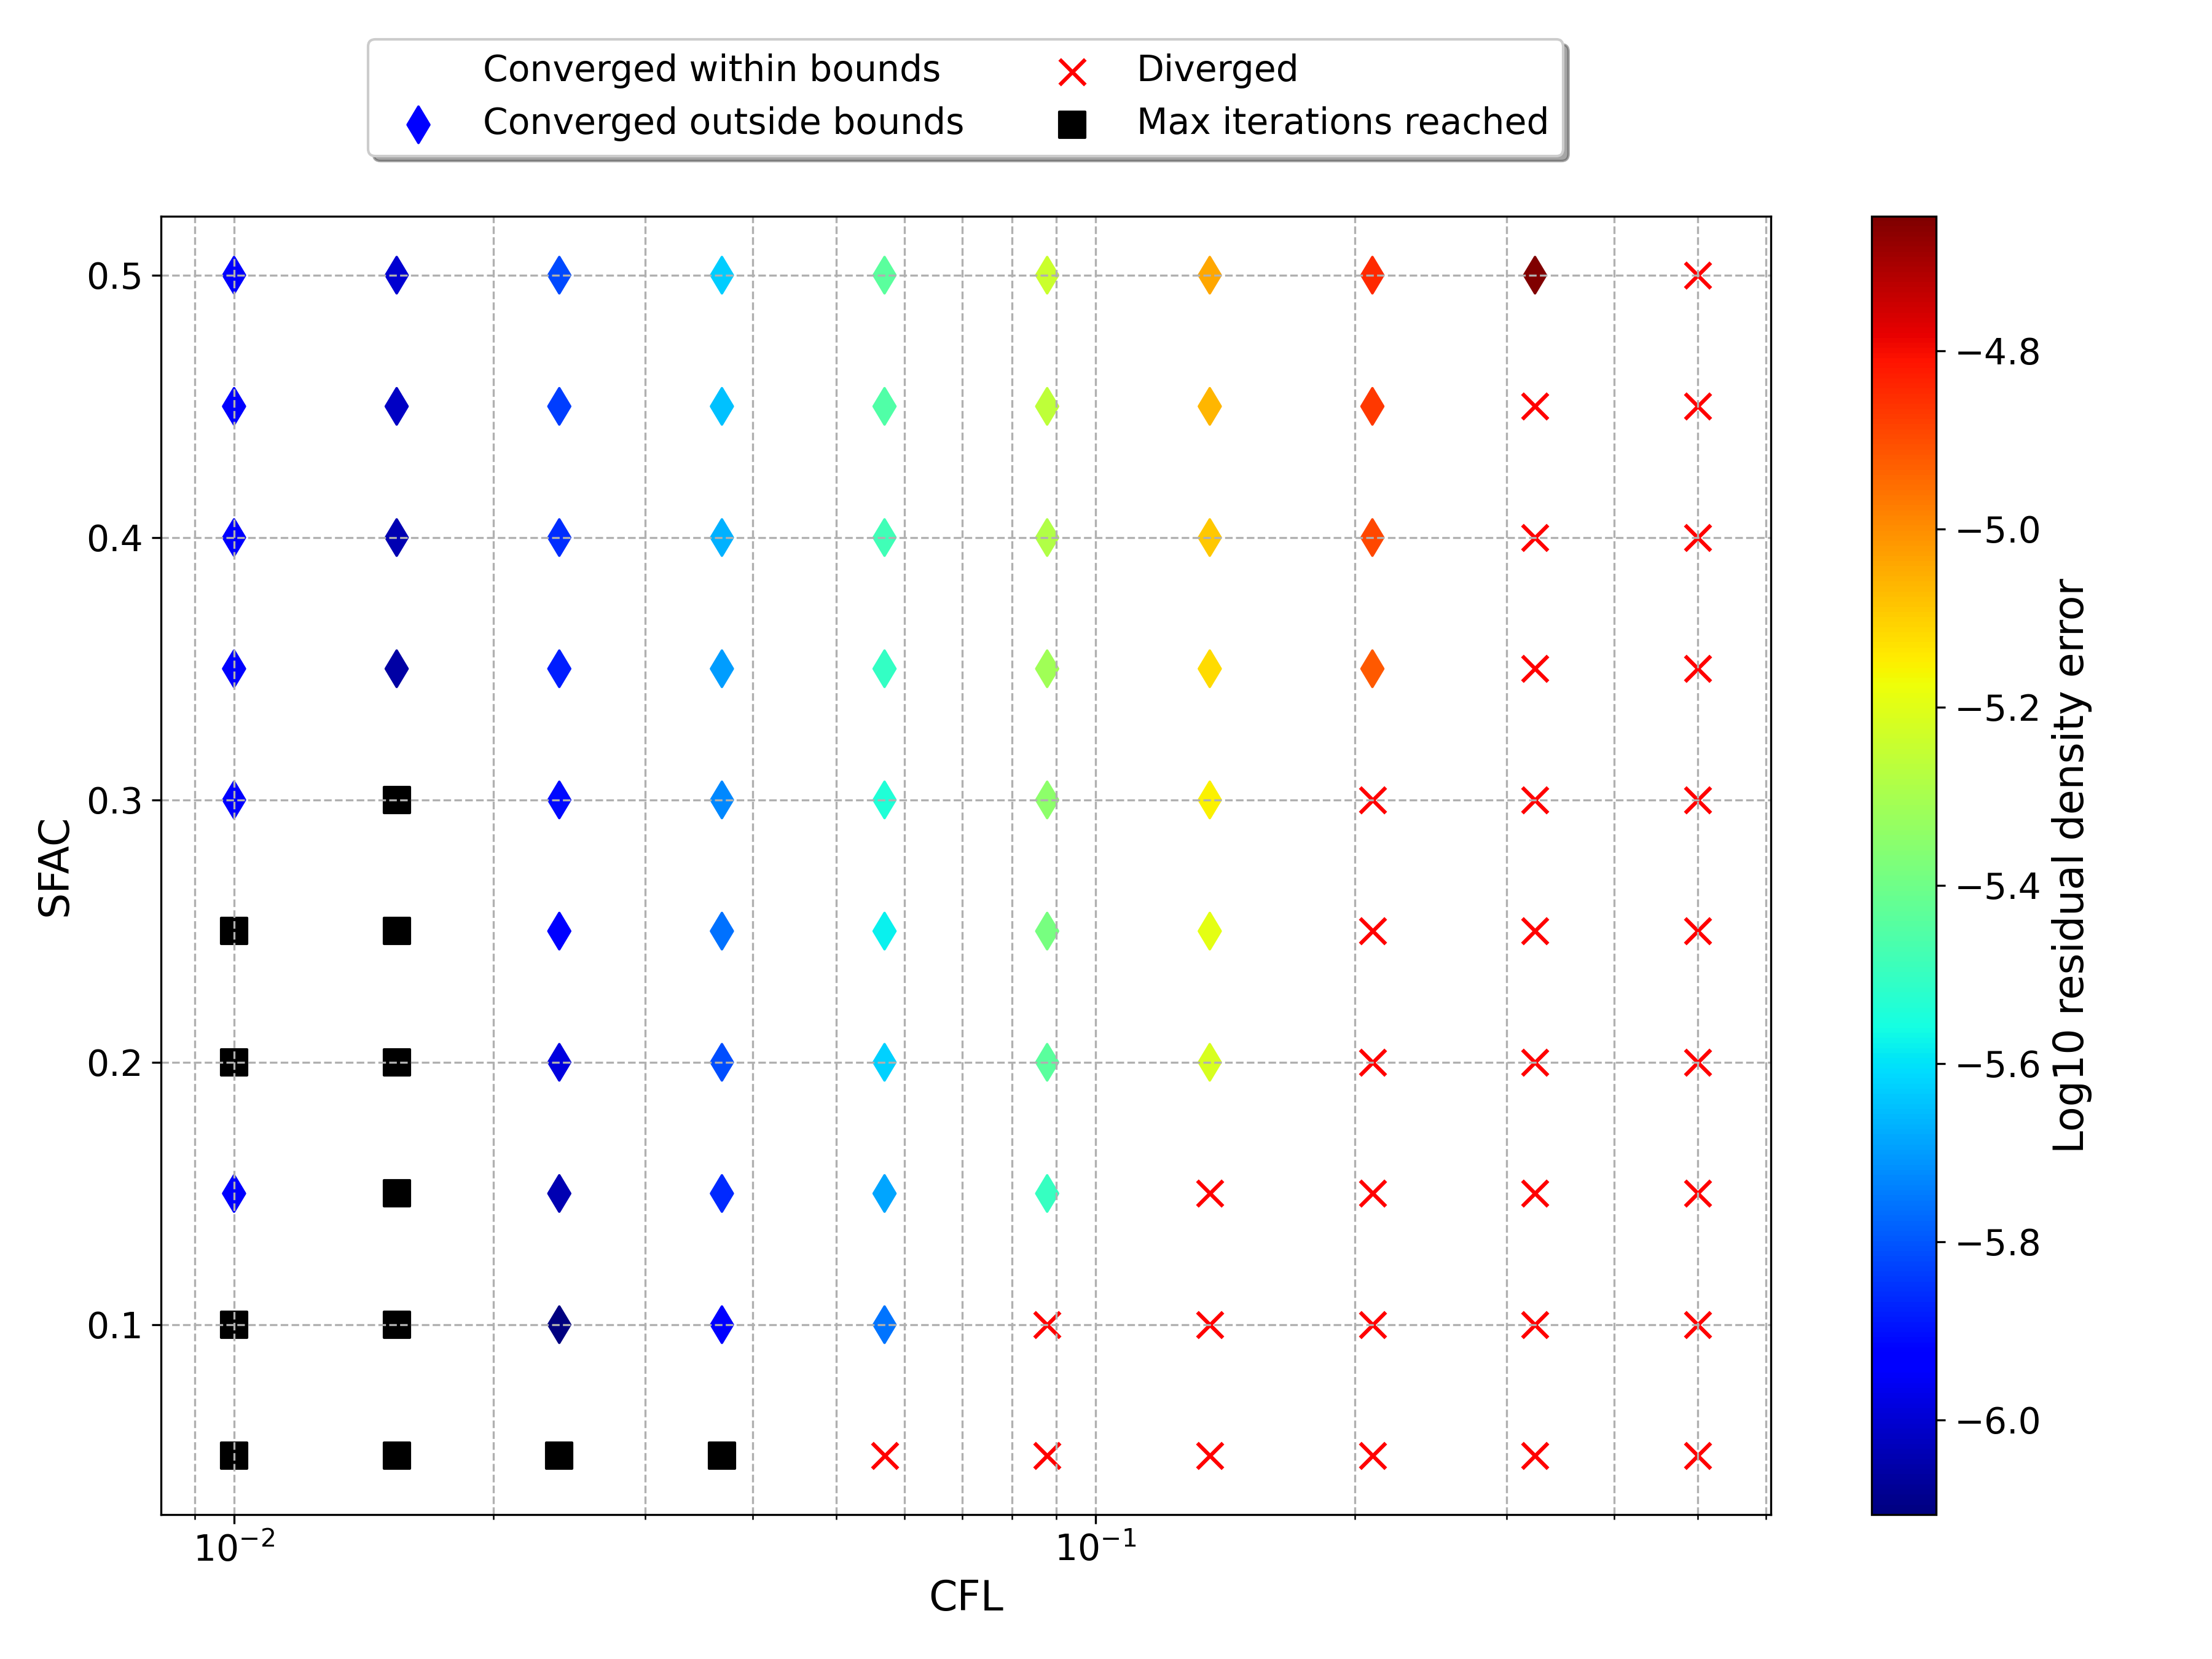
\includegraphics[width=0.8\textwidth]{figures/bend_cfl_sfac_residual.png}
    \caption{Scatter plot showing variation in residual error for different CFL and sfac values.}
    \label{fig:bend_cfl_sfac_residual}
\end{figure}

\begin{figure}[H]
    \centering
    \centering
    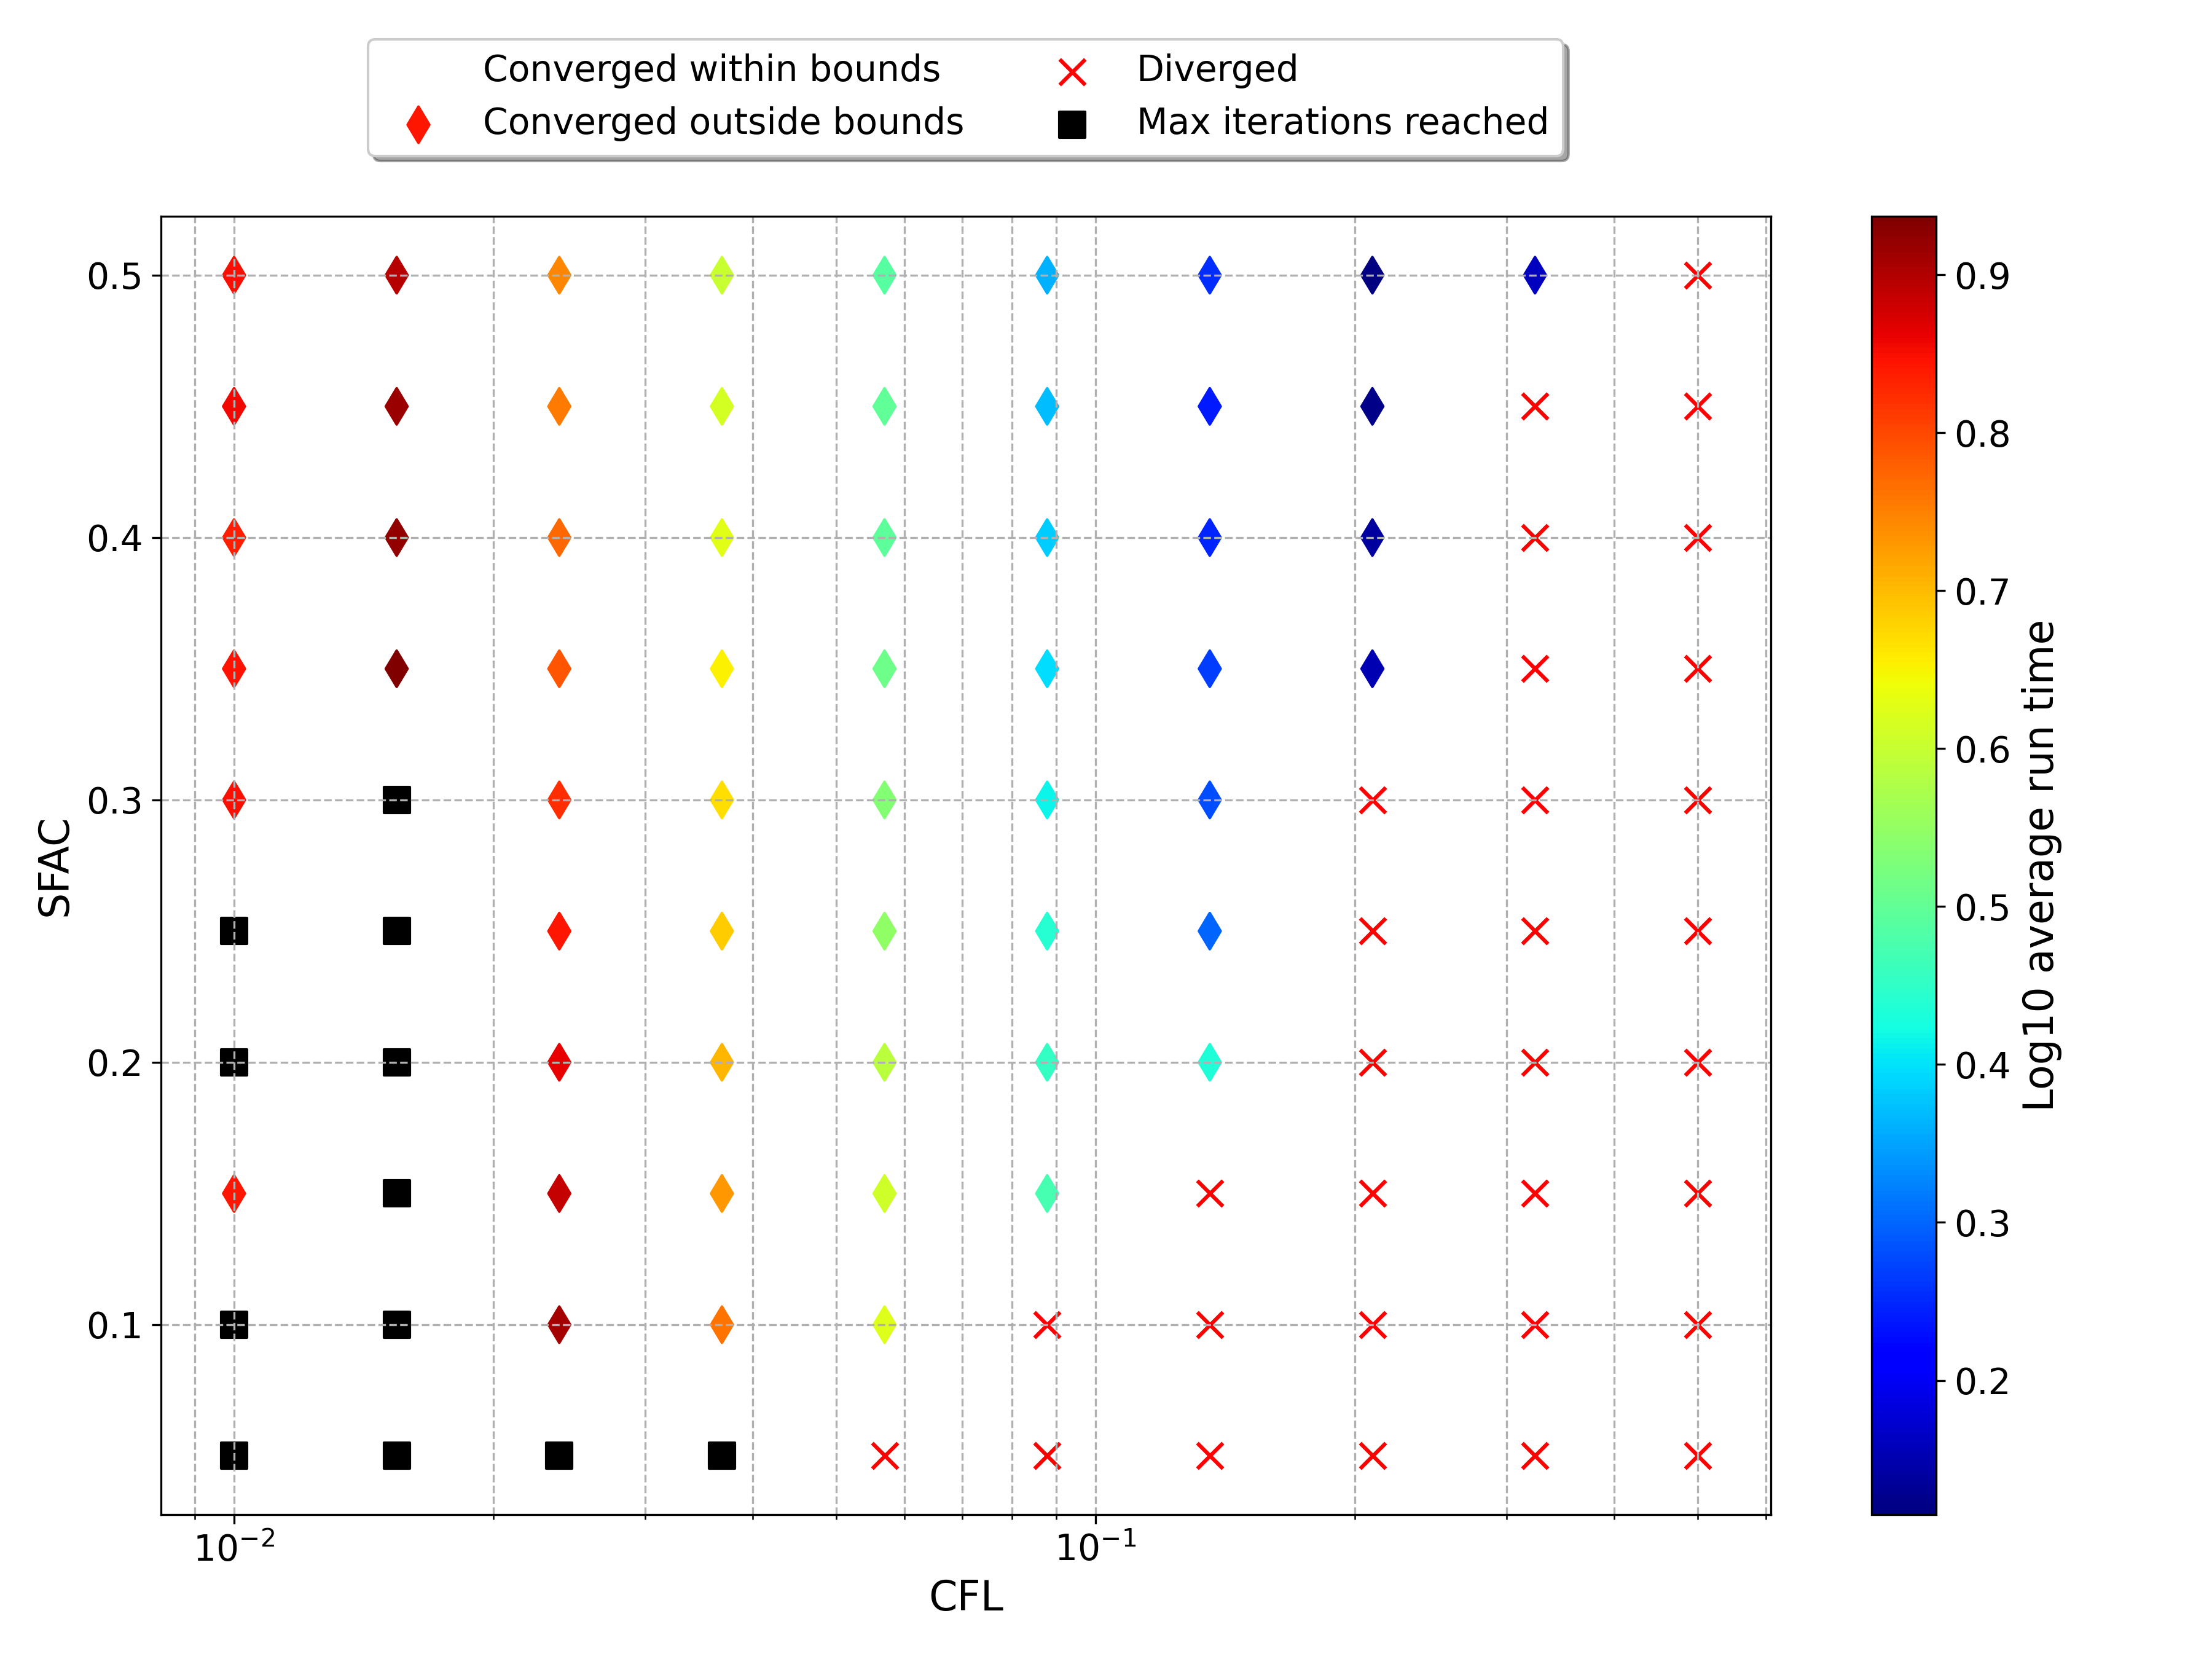
\includegraphics[width=0.8\textwidth]{figures/bend_cfl_sfac_time.png}
    \caption{Scatter plot showing variation in run time for different CFL and sfac values.}
    \label{fig:bend_cfl_sfac_time}
\end{figure}

\subsection{Comparison of compiler options }

\begin{table}[H]
    \centering
    \begin{tabular}{lcc}
        \toprule
        \textbf{Configuration} & \textbf{Normalised Time}\footnotemark  & \textbf{Variation Coefficient} \\
        \midrule
        Debug & 6.83 & 0.021 \\
        Release O2 & 1.05 & 0.018 \\
        Release O2, QxHost & 1.69 & 0.049 \\
        Release O2, Qparallel & 2.66 & 0.087 \\
        Release O2, fp:fast & 1.01 & 0.036 \\
        Release O3 & 1.09 & 0.016 \\
        Release O3, fp:fast & 1.00 & 0.010 \\
        Release O2 & 1.03 & 0.019 \\
        \bottomrule
    \end{tabular}
    \caption{Standard bump case run times for various compiler flags, normalised by the minimum averaged time. The average and deviation were found over three runs at a low $CFL$ such that 20,000 iterations were performed.}
    \label{tab:performance}
\end{table}


\begin{thebibliography}{9}

  \bibitem{handout}
  J. V. Taylor and J. C. Massey
  \emph{GA3 Heat Exchanger Handout}
  University of Cambridge,
  2024.

\end{thebibliography}

\end{document}